\documentclass[12pt,a4paper]{report}
\usepackage[english]{babel}
\usepackage[utf8x]{inputenc}
\usepackage{newlfont}
\usepackage{color}
\usepackage{hyperref}
\usepackage{amsmath}
\usepackage{graphicx}
\usepackage{epigraph}
\usepackage[overload]{empheq}
\usepackage[inline, shortlabels]{enumitem}
\usepackage{bm}
\usepackage[table]{xcolor}
\usepackage{color}
\usepackage{natbib}
\usepackage{float}
\usepackage{textcomp}
\usepackage{adjustbox}

\definecolor{grayrow}{rgb}{0.85, 0.85, 0.85}
\definecolor{lightgray}{rgb}{0.83, 0.83, 0.83}
\definecolor{darkgrayrow}{rgb}{0.7, 0.7, 0.7}
\definecolor{RoyalRed}{rgb}{0.61,0.11,0.19}

\usepackage{listings}

\definecolor{codegreen}{rgb}{0,0.6,0}
\definecolor{codegray}{rgb}{0.5,0.5,0.5}
\definecolor{codepurple}{rgb}{0.58,0,0.82}
\definecolor{backcolour}{rgb}{0.95,0.95,0.92}

\lstdefinestyle{snippet}{
    backgroundcolor=\color{backcolour},
    commentstyle=\color{codegreen},
    keywordstyle=\color{magenta},
    numberstyle=\tiny\color{codegray},
    stringstyle=\color{codepurple},
    basicstyle=\ttfamily\footnotesize,
    breakatwhitespace=false,
    breaklines=true,
    captionpos=t,
    keepspaces=true,
    numbers=left,
    numbersep=5pt,
    showspaces=false,
    showstringspaces=false,
    showtabs=false,
    tabsize=2
}

\usepackage{emptypage} % remove header in blanck pages

\usepackage[a4paper,top=4cm,bottom=4cm,left=3cm,right=3cm,marginparwidth=1.75cm]{geometry}

\hypersetup{
colorlinks,
citecolor=black,
filecolor=black,
linkcolor=black,
urlcolor=blue
}

\textwidth=450pt\oddsidemargin=0pt

\begin{document}
\begin{titlepage}
%
%
% ONCE YOU ARE FINISHED WITH YOUR CHANGES MODIFY "RED" WITH "BLACK" IN ALL \textcolor COMMENTS
%
%
\begin{center}
{{\Large{\textsc{Alma Mater Studiorum $\cdot$ University of  Bologna}}}} 
\rule[0.1cm]{15.8cm}{0.1mm}
\rule[0.5cm]{15.8cm}{0.6mm}
\\\vspace{3mm}
{\small{\bf School of Science \\
Department of Physics and Astronomy\\
Master Degree in Physics}}
\end{center}

\vspace{17mm}

\begin{center}
%
% INSERT THE TITLE OF YOUR THESIS
%
{\LARGE{\bf OPTIMIZATION AND APPLICATIONS\\
OF DEEP LEARNING ALGORITHMS\\
\vspace{3mm}
FOR SUPER-RESOLUTION IN MRI}}\\
\end{center}

\vspace{30mm} \par \noindent

\begin{minipage}[t]{0.47\textwidth}

{\large{\bf Supervisor: \vspace{2mm}\\
Prof. Gastone Castellani\\\\

\bf Co-supervisor:
\vspace{2mm}
\\
Dr. Nico Curti\\\\}}
\end{minipage}
%
\hfill
%
\begin{minipage}[t]{0.47\textwidth}\raggedleft \textcolor{black}{
{\large{\bf Submitted by:
\vspace{2mm}\\
Mattia Ceccarelli}}}
\end{minipage}

\vspace{40mm}

\begin{center}

Academic Year 2019/2020
\end{center}

\end{titlepage}

\newpage

\vspace*{125px}
\LARGE\textit{Abstract}
\normalsize
\vspace{2mm}

Abstract

\newpage
\normalsize 

\tableofcontents

\chapter{Introduction}

Brief introduction of the work

\section{Neural Network and Deep Learning}

  A neural network is an interconnected structure of simple procedurals units, called nodes. Their functionality is inspired by the animals' brain and from the works on learning and neural plasticity of Donald Hebb \cite{hebb-learning}. From his book :

\begin{quote}
 \begin{center}
  \textit{Let us assume that the persistence or repetition of a reverberatory activity (or "trace") tends to induce lasting cellular changes that add to its stability.[…] When an axon of cell A is near enough to excite a cell B and repeatedly or persistently takes part in firing it, some growth process or metabolic change takes place in one or both cells such that A's efficiency, as one of the cells firing B, is increased}
 \end{center}
\end{quote}

which is an attempt to describe the change of strenght in neural relations as a consequence of stimulations.
From the so-called \textit{Hebbian Theory} rose the first computational models such as the \textit{Perceptron}, \textit{Neural Networks} and the modern \textit{Deep Learning}. 
The development of learning-based algorithms didn't catch up with the expected results until recently, mainly due to the exponential increase in available computational resources.

From a mathematical point of view, a neural network is a composition of non-linear multi-parametric functions. 
During the {\it training phase} the model tunes its parameters, starting from random ones, by minimizing the error function (called also loss or cost). 
Infact, machine learning problems are just optimization problems where the solution is not given in an analytical form, therefore trough iteratives techniques (generally some kind of gradient descent) we progressively approximate the correct result.

In general, there are 3 different kind of approach to learning:

\begin{itemize}
 \item {\bf supervised} It exists a labeled dataset in which the relationship between features (input) and expected output is known. 
 During training, the model is presented with many examples and it corrects its answers based on the correct response.  
 Some problems tied to supervised algorithms are classification, regression, object detection, segmentation and super-resolution.
 \item {\bf unsupervised} In this case, a labeled dataset does not exist, only the inputs data are available. 
 The training procedure must be tailored around the problem under study. Some examples of unsupervised algorithms are clustering, autoencoders, anomaly detection.
 \item {\bf reinforced} the model interacts with a dynamic environment and tries to reach a goal (e.g. winning in a competitive game). 
 For each iteration of the training process we assign a reward or a punishent, relatively to the progress in reaching the objective.
\end{itemize}

This work will focus on models trained using labeled samples, therefore in a supervised environment.

\subsection*{Perceptron}

The Perceptron (also called \textit{artificial neuron}) is the fundamental unit of every neural network and it is a simple model for a biological neuron, based on the works of Rosenblatt \cite{perceptron}. 
The \textit{perceptron} receives $N$ input values $x_1, x_2, ... x_N$ and the output is just a linear combination of the inputs plus a bias :

\begin{equation}
y = \sigma(\sum_{k=1}^N w_kx_k + w_0)
\end{equation}

where $\sigma$ is called \textit{activation function} and $w_0, w_1, ... w_N$ are the trainable weights.

Originally, the activation function was the \textit{Heaviside step function} whose value is zero for negative arguments and one for non-negative arguments: 

\begin{equation}
H(x) := 
\begin{cases}
  0 \text{ if } x < 0 \\ 
  1 \text{ if } x \geq 0 \\
\end{cases}
\end{equation}

In this case the perceptron is a \textit{linear discriminator} and as such, it is able to learn an hyperplane which linearly separates two set of data.
The weights are tuned during the training phase following the given update rule, usually :

\begin{equation}
 \bm{w}_{n+1} = \bm{w}_n + \eta (t - y)\bm{x}
 \label{eq:perceptron}
\end{equation}

where $\eta$ is the learning rate ($\eta \in [0,1]$) and $t$ is the true output. If the input instance is correctly classified,  the error $(t - y)$ would be zero and no weight is changed. 
Otherwise, the hyperplane is moved towards the misclassified example. 
Repeating this process will lead to a convergence only if the two classes are linearly separable.  

\subsection*{Fully Connected Structure}

The direct generalization of a simple perceptron is the \textit{Fully Connected Artificial Neural Network} (or {\it Multy Layer Perceptron}). 
It is composed by many Perceptron-like units called nodes, any one them performs the same computation as formula \ref{eq:perceptron} and \textit{feed} their output \textit{forward} to the next layer of nodes. 
A typical representation of this type of network is shown in figure \ref{fig:ann}:

\begin{figure}[h]
 \centering
 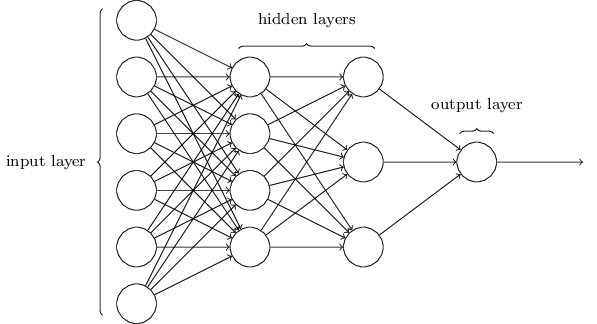
\includegraphics[scale=0.5]{./images/neural_net.png}
 \caption{{\it A common representation of a neural network: a single node works as the perceptron described above.}}
 \label{fig:ann}
\end{figure}

While the number of nodes in the input and output layers is fixed by the data under analysis, the best configuration of hidden layers is still an open problem.

The mathematical generalization from the perceptron is simple, indeed given the $i$-th layer its output vector $\bm{y}_i$ reads:  

\begin{equation}
 \bm{y}_i = \sigma(W_i \bm{y}_{i-1} + \bm{b}_i)
\end{equation}

where $W_i$ is the weights matrix of layer $i$ and $\bm{b}_i$ is the $i$-th bias vector, equivalent to $w_0$ in the perceptron case.
The output of the $i$-th layer becomes the input of the next one until the output layer yields the network's answer. 

As before, $\sigma$ is the activation function which can be different for every node, but it usually differs only from layer to layer. 
The choice of the best function for a given problem is still an open issue.

In a supervised environment, the model output is compared to the desired output ({\it truth}) by means of a cost function. 
An example of cost function is the sum of squared error : 

\begin{equation}
  C(W) = \frac{1}{N} \sum_{j=1}^{N} (y_j - t_j)^2
\end{equation}

where $N$ is the dimensionality of the output space. $C$ is considered as a function of the model's weights only since input data and true label $t$ are fixed.

Those architectures are {\it universal approximators}, that means given an arbitrarly complex function, there is a fully connected neural network that can approximate it.

This type of network is called {\it feed forward} because the information flows linearly from the input to the output layer: however, it exists a class of models called {\it Recurrent} where this is not the case anymore and feedback loop are possible, but they are outside the scope of this work. 

\subsection*{Gradient Descent}

To minimize the loss function an update rule for the weights is needed. 
Given a cost funtion $C(w)$, the most simple one is the gradient descent:
\begin{equation}
 w \leftarrow w - \eta \nabla_w C
\end{equation}
The core idea is to modify the parameters by a small step in direction that minimize the error function. 
The lenght of the step is given by the {\it learning rate} $\eta$, which is a hyperparameter chosen by the user, while the direction of the step is given by $-\nabla_w C$, which point towards the steepest descent of the function landscape.

\begin{figure}[h]
 \centering
 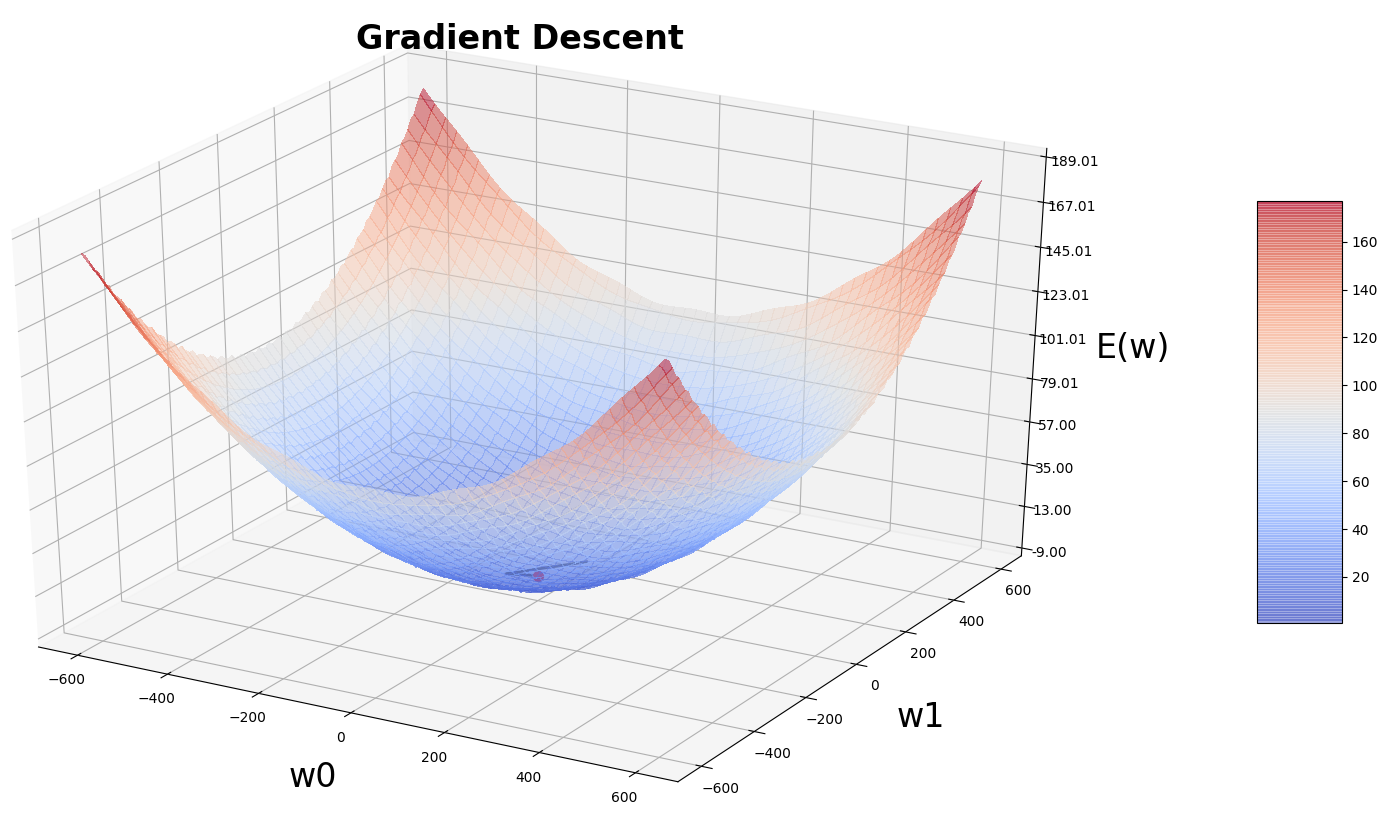
\includegraphics[scale=0.8]{./images/sgd.png}
 \caption{\it Visual example of gradient descent for a model with 2 weights. The idea is to modify the weights to follow the direction of steepest descent for the landscape of the error function}
 \label{fig:gd}
\end{figure}
The speed at which the algorithm converge to a solution and the precision of said solution are greatly influenced by the update rule. More complex and efficient update rules do exist, but they follow the same idea as the gradient descent.

\subsection*{Error Back Propagation}

The most common algorithm used to compute the updates to weights in the learning phase is the {\it Error Back Propagation}. 
Given a differentiable cost function $C(W)$, let's define :
\begin{align}
 \bm{z}_l &= W_l \bm{y}_{l-1} + \bm{b}_l  \\ 
 \bm{a}_l &= \sigma(\bm{z}_l)
\end{align}
respectively the de-activated and activated output vectors of layer $l$ for a model with $L$ total layer, and:
\begin{equation}
 \bm{\delta}_l = (\frac{\partial C}{\partial z_l^1}, \dots , \frac{\partial C}{\partial z_l^N}) 
\end{equation}
as the vector of errors of layer $l$. Then we can write the 4 equations of back propagation for the fully connected neural network \cite{neural-net-nielsen}:
\begin{align}
  &\bm{\delta}_L = \nabla_a C \odot \sigma'(\bm{z}_L) \\ 
  &\bm{\delta}_l = (W_{l+1}^T \bm{\delta}_{l+1}) \odot \sigma'(\bm{z}_l) \\
  &\frac{\partial C}{\partial b_l^j} = \delta_l^j \\
  &\frac{\partial C}{\partial w_l^{j k}} = a_{l-1}^k \delta_{l}^{j}
\end{align}
where  $\odot$ is the element-wise product.
Those equations can be generalized for others kind of layer, as I will show in the next chapters. 

The full training algorithm is : 

\begin{itemize}
 \setlength\itemsep{-0.3em}
 \item [-] define the model with random parameters
 \item [-] compute the output for one of the inputs
 \item [-] compute the loss function $C(W)$ and the gradients $\frac{\partial C}{\partial w_l^{j k}}$ and $\frac{\partial C}{\partial b_l^j}$ for each $l$.
 \item [-] updates the parameters following the update rule, 
 \item [-] iterate from step 2 until the loss is sufficiently small
\end{itemize}

\section{Super Resolution}

The term Super-Resolution (SR) referes to a class of techniques which aim is to enhance the spatial resolution of an image, thus converting a given low resolution (LR) image to a corresponding high resolution (HR) one, with better visual quality and refined details.
Image super-resolution is also called by other names like image scaling, interpolation, upsampling and zooming \cite{survey-sr}.
Super resolution can also refers to its "hardware" (and best-known) implementation, the {\it super resolution microscopy}, which aim is to overcome the diffraction limit: indeed, the development of super-resolved fluorescense microscopy won a Nobel price in chemistry in 2014, though its technicalities reside outside the scope of this work, which focused on its numerical counterpart.

As described before, the training of a supervised model happens by means of examples: in the case of classification the network is presented with many couples {\it features-label} that compose the {\it train set}. The objective is find the correct label for a set of sample never saw before called {\it test set}.

For digital images, the {\it features} are the pixels which compose a 2 dimensional or 3 dimensional (for RGB picture) grid-like structure, the label is usually represented as 1 dimensional vector as large as the binary representation of the number of classes the model is supposed to  discern: a neural network produces a map between a very large {\it features space} and a smaller one.

This behaviour is slightly different for Super-Resolution: indeed, when training a SR model we are talking about {\it image-to-image} processing and as such, both the features space and the labels are images.  
The dataset is built from a single series of high resolution (HR) images which are downsampled to obtain the low resolution (LR) counterpart: the couples LR-HR are fed to the network respectively as input and label just like in a classification problem; this time though, the network will map a smaller feature space into a larger one. 

The models I'm going to use in this work are trained on images downsampled using the {\it bicubic interpolation}.


\subsection{Bicubic Interpolation}

The {\it Bicubic interpolation} is a common algorithm used in image analysis either to downsample or upsample an image. 
This operation is also called \textit{re-scaling} and its purpose is to interpolate the pixel values after a resize of the image, respectively after shrinking or expanding it, e.g as a consequence of zooming. 
The name comes from the highest order of complexity of the operation used in the algorithm, which is a cubic function. 
Given a pixel, the interpolation function evaluates the 4 pixel around it by applying a filter defined as:

\begin{equation}
\hspace*{-1.cm}
k(x) = \frac{1}{6} \left\{ \begin{array}{rc}
  (12 - 9B - 6C) |x|^3 + (-18 + 12B + 6C) |x|^2 + (6 - 2B)           & \mbox{if }        |x| < 1 \\
  (−B − 6C) |x|^3 + (6B + 30C) |x|^2 + (−12B − 48C) |x| + (8B + 24C) & \mbox{if } 1 \leq |x| < 2 \\
  0                                                                  & \mbox{otherwise}         \\
  \end{array}
  \right.
\end{equation}
 
where $x$ identifies each pixel below the filter.
Common values used for the filter parameters are $B=0$ and $C=0.75$ (used by \textsf{OpenCV} library) or $B=0$ and $C=0.5$ used by \textsf{Matlab}.
The scale factor of the down/up sampling can assume different values according to the user needs; for this work, I used an upsampling factor of $\times 2$ and $\times 4$ and the algorithm is from the \textsf{Python} version of the library \textsf{OpenCV} \cite{OpenCV}. 
The main aims of SR algorithms are to provide a better alternative to standard upsampling and obtain a better quality image both from a qualitative (visual perception) and a quantitative poin of view. 

\subsection{Image Quality}

While the human eye is a good qualitative evaluator, it is possible to define different quantitative measures between two images to quantify their similiraties.

\subsection*{PSNR}

One of the most common in Image Analysis is the {\it Peak Signal To Noise Ratio} or PSNR. 
It is usually employed to quantify the recostruction capabilities of an algorithm given a lossy compression, w.r.t the original image. The mathematical espression reads: 

\begin{equation}
 PSNR = 20 \cdot \log_{10} (\frac{max(I)}{MSE})
\end{equation}

where $max(I)$ is the maximum available value for the image $I$, namely $1$ for floating point representation and $255$ for an integer one. 
$MSE$ is the {\it Mean Squared Error}, which is a common metrics in data analysis used to quantify the mean error of a model. It's defined as:

\begin{equation}
 MSE = \frac{1}{HW}\sum_{i=1}^{H} \sum_{j=1}^W (I(i, j) - K(i,j))^2
\end{equation}
 
where $H$ and $W$ are the spatial dimensions of the original image $I$ and the recostruction $K$. 
The metric can be generalized to colored image by simply adding the depth (RGB channel) dimension.

Even though an higher PSNR generally means an higher recostruction quality, this metric may performs poorly compared to other quality metrics when it comes to estimate the quality as perceived by human eyes. An increment of $0.25$ in PSNR corresponds to a visible improvement.
 
\subsection*{SSIM}

Another common metric is the {\it Structural SIMilarity index} or SSIM. It has been developed to evaluate the structural similraties between two images,  while incorporating important perceptual phenomena, including luminance and contrast terms. For that, it should be more representative of the qualitative evaluation as seen by humans.
The SSIM index is defined as: 

\begin{equation}
 SSIM(I, K) = \frac{1}{N} \sum_{i=1}^{N} SSIM(x, y)
\end{equation}

Where $N$ is the number of windows in the images, usually of size $11 \times 11$ or $8 \times 8$. For every box, the index is : 

 \begin{equation}
    \hspace{-0.75cm}
    SSIM(x, y) = \frac{1}{N}\sum_{i=1}^{N} \frac{(2\mu_x\mu_y + c_1)(2\sigma_{xy} + c_2)}{ ({\mu_x}^2 + {\mu_y}^2 + c_1)({\sigma_x}^2 + {\sigma_y}^2 + c_2) },
    \label{SSIM}
\end{equation}

where $x$ and $y$ are two equally-sized regions in two different images, $\mu$ is the average value in the region, $\sigma^2$ is the variance, $\sigma_{xy}$ is the covariance between the regions and $c_1$ and $c_2$ are two constants to stabilize the division.

Both SSIM and PSNR can be useful in Deep Learning applications as target functions or as post-training quality measures. 
To compute PSNR and SSIM I used the function of the Python library {\it scikit image} \cite{scikit}, for their precision, efficency and ease to use.

SR pre-trained models will be evaluated in their reconstruction capabilities against the bicubic interpolation using as benchmark an available dataset of NMR images of brain. 
I'd like to point out that the deep learning architecture tested in this work are trained  on general purpose datasets which are very different from biomedical pictures available:  the first problem is that MRI images are single channeled (gray-scaled) as opposed to the RGB images which those models are trained on, however this can be easily solved by artificially add depth by concatenating the same image 3 times; by doing so, the models elaborate tree different outputs that can be compared against each others.  
The second issue is that the models never had a chance to learn the particular shapes contained in animals' brain: although that could be seen as a major drawback, their generalization capability should be sufficient to perform well even outside their optimal "environment". 
The datasets will be discussed in later chapters.

\section{Magnetic Resonance}

\chapter{Algorithms}

A wide range of documentations and implementations have been written on the topic of Deep Learning and it is more and more difficult to move around the different sources.
In recent years, leaders in DL applications became the multiple open-source \textsf{Python} libraries available on-line as \textsf{Tensorflow}~\cite{tensorflow2015-whitepaper}, \textsf{Pytorch}~\cite{paszke2017automatic} and \textsf{Caffe}~\cite{Jia:2014:Caffe}.
Their portability and efficiency are closely related on the simplicity of the \textsf{Python} language and on the simplicity in writing complex models in a minimum number of code lines.
Only a small part of the research community uses deeper implementation in \textsf{C++} or other low-level programming languages and between them should be mentioned the \textsf{darknet project} of Redmon J. et al. which has created a sort of standard in object detection applications using a pure \textsf{Ansi-C} library.
The library was developed only for Unix OS but in its many branches (literally \emph{forks}) a complete porting for each operative system was provided.
The code is particularly optimized for GPUs using CUDA support, i.e only for NVidia GPUs.
It is particularly famous for object detection applications since its development is tightly associated to an innovative approach at multi-scale object detections called YOLO (\emph{You Only Look Once}), that recently reached its fourth release \cite{yolov4}.
The libraries built during the develompment of this thesis are all inspired by the efficiency and modularity of darknet and make an effort to not only replicate but expand on their work, both in performances, functionalities and solved issues.

In this section I will describe the mathematical background of these models and 
to most theoretical explanation  discuss the numerical problems associated, tied to the development of two new libraries: \textsf{NumPyNet} \cite{NumPyNet} and \textsf{Byron} \cite{Byron}.

\section{Frameworks}

\textsf{NumPyNet} is born as an educational framework for the study of Neural Network models.
It is written trying to balance code readability and computational performances and it is enriched with a large documentation to better understand the functionality of each script.
The library is written in pure \textsf{Python} and the only external library used is \textsf{Numpy}~\cite{Numpy} (a base package for the scientific research).
As I will show in the next sections, \textsf{Numpy} allows a relatively efficient implementation of complex algorithms by keeping the code as similar as possible to the mathematic computations involved.

Despite being supplied by wide documentations, it is often difficult for novel users to move around the many hyper-links and papers cited in all common libraries.
\textsf{NumPyNet} tries to overcome this problem with a minimal mathematical documentation associated to each script and a wide range of comments inside the code.

An other "problem" to take into account is associated to performances.
On one hand, libraries like \textsf{Tensorflow} are certainly efficient from a computational point-of-view and the numerous wraps (like \emph{Keras}) guarantee an extremely simple user interface.
On the other hand, the deeper functionalities of the code and the implementation strategies used are unavoidably hidden behind tons of code lines.
In this way the user can perform complex computational tasks using the library as black-box package.
\textsf{NumPyNet} wants avoid this problem using simple \textsf{Python} codes, with extreme readability also for new users, to better understand the symmetry between mathematical formulas and code.
The simplicity of this library allows us to give a first numerical analysis of the model functions and, moreover, to show the results of each function on an image to better understand the effects of their applications on real data.
Each \textsf{NumPyNet} function was tested against the equivalent \textsf{Tensorflow} implementation, using an automatic testing routine through \textsf{PyTest}~\cite{PyTest}.
The full code is open-source on the \textsf{Github} page of the project.
Its installation is guaranteed by a continuous integration framework of the code through \textsf{Travis CI} for Unix environments and \textsf{Appveyor CI} for Windows OS.
The library supports \textsf{Python} versions $\ge2.6$.

As term of comparison we discuss the more sophisticated implementation given by the \textsf{Byron} library.
\textsf{Byron} (\emph{Build YouR Own Neural network}) library is written in pure \textsf{C++} with the support of the modern standard \textsf{C++17}.
We deeply use the \textsf{C++17} functionality to reach the better performances and flexibility of our code.
What makes \textsf{Byron} an efficient alternative to the competition is the complete multi-threading environment in which it works.
Despite the most common Neural Network libraries are optimized for GPU environments, there are only few implementations which exploit the full set of functionalities of a multiple CPUs architecture.
This gap discourages multiple research groups on the usage of such computational intensive models in their applications.
\textsf{Byron} works in a fully parallel section in which each single computational function is performed using the entire set of available cores.
To further reduce the time of thread spawning, and so optimize as much as possible the code performances, the library works using a single parallel section which is opened at the beginning of the computation and closed at the end.

The \textsf{Byron} library is released under \textsf{MIT} license and publicly available on the \textsf{Github} page of the project.
The project includes a list of common examples like object detection, super resolution, segmentation.
The library is also completely wrapped using \textsf{Cython} to enlarge the range of users also to the \textsf{Python} ones.
The complete guide about its installation is provided; the installation can be done using \textsf{CMake}, \textsf{Make} or \textsf{Docker} and the \textsf{Python} version is available with a simple \textsf{setup.py}.
The testing of each function is performed using \textsf{Pytest} framework against the \textsf{NumPyNet} implementation (faster and lighter to import than \textsf{Tensorflow}) \cite{nicotesi}.

\section{Convolutional Neural Network}

A Convolutional Neural Network (CNN) is a specialized kind of neural network for processing data that has known grid-like topology \cite{Goodfellow-et-al-2016}, like images, that can be considered as a grid of pixels.
The name indicates that at least one of the functions employed by the network is a convolution. In a continuos domain the convolution between two functions $f$ and $g$ is defined as: 
\begin{equation}
 (f * g)(t) = \int_{-\infty}^{+\infty} f(\tau)g(t-\tau)d\tau
\end{equation}
The first function $f$ is usually referred to as the input and the second function $g$ as kernel. 
For Image Processing applications we can define a 2-dimensional discrete version of the convolution in a finite domain using an image $I$ as input and a 2 dimensional kernel $k$:
\begin{equation}
 C[i, j] = \sum_{u=-N}^N \sum_{v=-M}^M k[u, v] \cdot I[i-u, j-v]
 \label{eq:conv}
\end{equation}
where $C[i, j]$ is the pixel value of the output image and $N$, $M$ are the kernel dimensions.
Practically speaking, a convolution is performed by sliding a kernel of dimension $N \times M$ over the image, each kernel position corresponds to a single output pixel, the value of which is calculated by multiplying together the kernel value and the underlaying pixel value for each cell of the kernel and summing all the results, as shown in figure \ref{fig:convolution}:

\begin{figure}[h]
 \centering
 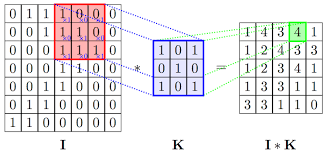
\includegraphics[scale=1.]{./images/conv.png}
 \caption{\it Visual example of convolution of an image I 7x7 with a 3x3 kernel K.}
 \label{fig:convolution}
\end{figure}

The convolution operation is also called $filtering$. By chosing the right kernel (filter) it is possible to highlight different features. For this reason the convolution operation is commonly used in image analysis: some of the most common applications are denoising, edge detection and edge enhancement. 

\section{Layers}

As described above, a neural network can be considered as a composition of function: for this reason every Deep Learning framework (e.g. Keras/Tensorflow, Pytorch, Darknet) implement each function as an independent object called {\it Layer}. In Byron and NumPyNet, each layer contains at least 3 methods:
\begin{itemize}
 \setlength\itemsep{-0.3em}
 \item {\bf forward} the forward method compute the output of the layer, given as input the previous output. 
 \item {\bf backward} the backward method is essential for the training phase of the model: indeed, it computes all the updates for the layer weights and backpropagates the error to the previous layers in the chain.
 \item {\bf update} the update method applies the given update rules to the layer's weights.
\end{itemize}
By stacking different kinds of layer one after another, it is possible to build 
complex models with tens of millions of parameters. 
For the purposes of this work, I'm going to describe layers used in super resolution, however, Byron is developed also for different applications (object detection, classification, segmentation, style transfer, natural language processing etc...) and as such, many more layers are available.   

\subsection*{Convolutional Layer}

The convolutional layer (CL) object is the most used layer in DL image analysis, therefore its implementation must be as efficient as possible.
Its purpose is to perform multiple (sometimes thousands) convolution over the input to extract different high-level features, which are compositions of many low-level attributes of the image (e.g edges, simple shapes).
In the brain/neuron analogy, every entry in the output volume can also be interpreted as an output of a neuron that looks at only a small region, the neuron's {\it receptive field} in the input and shares parameters with all the neuron spatially close.
As more CLs are stacked, the receptive field of a single neuron grows and with that, the complexity of the features it is able to extract.
The local nature of the receptive field allows the models to recognize features regardless of the position in the images. In other words, it is independent from translations \cite{Goodfellow-et-al-2016}. 

The difference from a traditional convolutional approach is that instead of using pre-determined filters, the network is supposed to learn its own.
A CL si defined by the following parameters: 

\begin{itemize}
 \setlength\itemsep{-0.2em}
 \item [-] {\bf kernel size} : it is the size of the sliding filters. The depth of the filters is decided by the depth of the input images (which is the number of channels.). The remanining 2 dimensions (widht and height) can be indipendent from one another, but most implementation require square kernels.
 \item [-] {\bf strides} : defines the movement of the filters. With a low stride (e.g. unitary) the windows tends to overlap. With highr stride values we have less overlap (or none) and the dimension of the output decrease.
 \item [-] {\bf number of filters} : is the number of different filters to apply to the input. It also indicates the depth of the output.
 \item [-] {\bf padding} : is the dimensions of an artificial enlargement of the input to allow the application of filters on borders. Usually, it can be interpreted as the number of rows/columns of pixel to add to the input, however some libraries (e.g Keras) consider it only as binary: in case is true, only the minimum number of rows/columns are appended to keep the same spatial dimension.
\end{itemize}
Given the parameters, it is straightforward to compute the number of weights and bias needed for the initialization of the CL: indeed, suppose an image of dimensions $(H, W, C)$ slided by $n$ different 3-D filters of size $(k_x, k_y)$ with strides $(s_x, s_y)$ and padding $p$, then:
\begin{align}
 \# weights &= n \times k_x \times k_y \times C \\
 \# bias &= n
\end{align}
Note that the number of weights does not depend on the input spatial size but only on its depth. It is important because a fully convolutional network can receives images of any size as long as they have the correct depth. Moreover, using larger inputs do not requires more weights, as is the case for fully connected structure. 

The output dimensions are $(out\_H, out\_W, n)$ where :
\begin{align}
 out\_H &= \lfloor\frac{H - k_x + p}{s_x}\rfloor + 1 \\
 out\_W &= \lfloor\frac{W - k_y + p}{s_y}\rfloor + 1
\end{align}

Even if the operation can be implemented as described above in equation \ref{eq:conv}, this is never the case: it is certainly easier but also order of magnitude slower than more common algorithms.
A huge speed up in performances is given by realising that a discrete convolution can be viewed as a single matrix multiplication. By performing a clever transformation of the input into a flat matrix, in which every columns yields the values that have to be multiplied by the filters for each output, as shown in figure \ref{fig:im2col}

\begin{figure}[h]
 \centering
 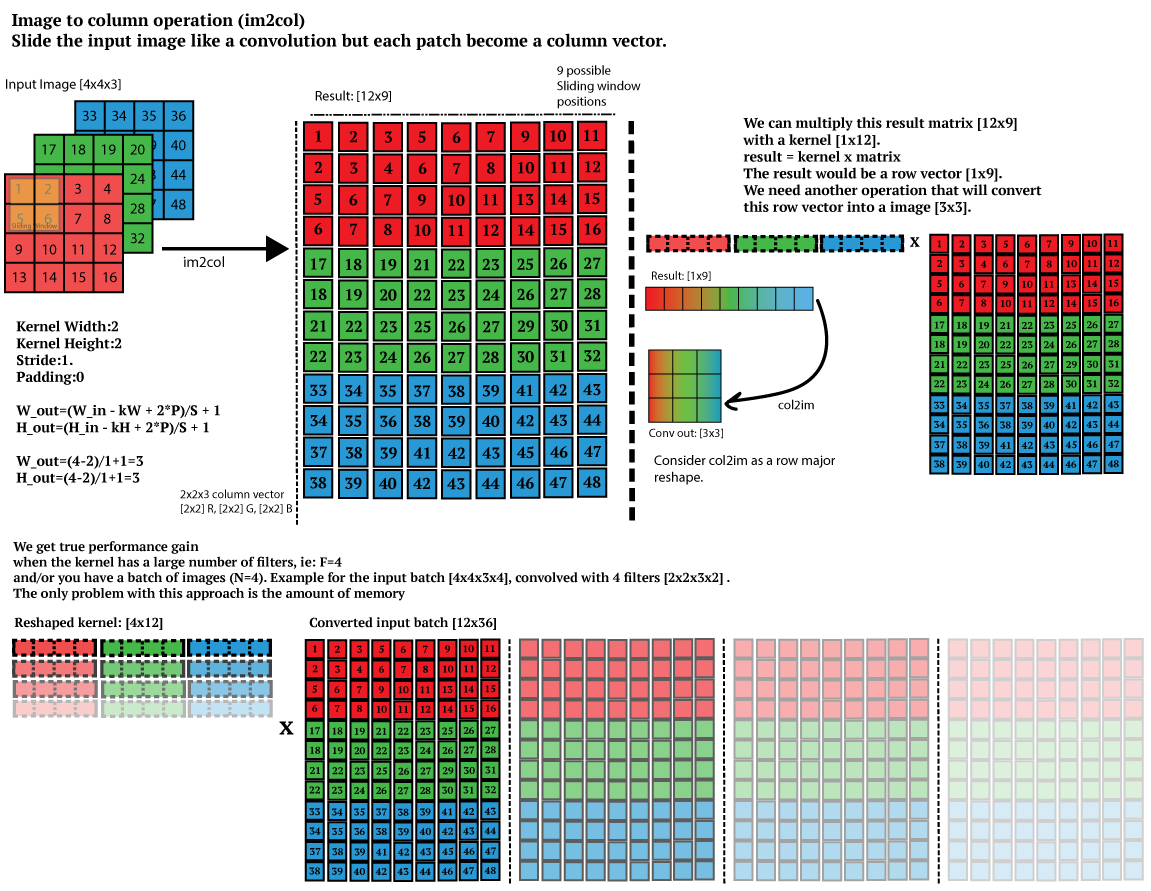
\includegraphics[scale=0.35]{./images/im2col.png}
 \caption{\it Scheme of the im2col algorithm using a $2 \times 2 \times 3$ filter with stride 1 on a $4 \times 4 \times 3$ image. The matrix multiplication is between a $n \times 12$ and a $12 \times 9$ matrixes.}
 \label{fig:im2col}
\end{figure}

This re-arrengement is commonly called im2col. The main downside is that a lot more memory is needed to store the newly arranged matrix.
The larger the number of kernels, the higher is the time gain of this implementation over a naive one.  

Another important optimization comes from linear algebra considerations and is called {\it Coppersmith-Winograd algorithm}, which was designed to optimize the matrix product.
Suppose we have an input image of just 4 elements and a 1-D filter mask with size 3:

\begin{equation}
\mbox{img} = \left[\begin{array}{cccc} d0 & d1 & d2 & d3 \end{array}\right] \quad\quad \mbox{weights} = \left[\begin{array}{ccc} g0 & g1 & g2 \end{array}\right]
\end{equation}
\\
we can now use the \textsf{im2col} algorithm previously described and reshape our input image and weights into

\begin{equation}
\mbox{img} = \left[
\begin{array}{ccc}
d0 & d1 & d2 \\
d1 & d2 & d3
\end{array}
\right],
\quad\quad
\mbox{weights} = \left[
\begin{array}{c}
g0 \\
g1 \\
g2
\end{array}
\right]
\end{equation}
\\
given this data, we can simply compute the output as the matrix product of this two matrices:

\begin{equation}
\mbox{output} = \left[
\begin{array}{ccc}
d0 & d1 & d2 \\
d1 & d2 & d3
\end{array}
\right]
\left[
\begin{array}{c}
g0 \\
g1 \\
g2
\end{array}
\right] = \left[
\begin{array}{c}
d0 \cdot g0 + d1 \cdot g1 + d2 \cdot g2 \\
d1 \cdot g0 + d2 \cdot g1 + d3 \cdot g2 
\end{array}
\right]
\end{equation}
\\
The Winograd algorithm rewrites this computation as follow:

\begin{equation}
\mbox{output} = \left[
\begin{array}{ccc}
d0 & d1 & d2 \\
d1 & d2 & d3
\end{array}
\right]
\left[
\begin{array}{c}
g0 \\
g1 \\
g2
\end{array}
\right] = \left[
\begin{array}{c}
m1 + m2 + m3 \\
m2 - m3 - m4
\end{array}
\right]
\end{equation}
\\
where

\begin{equation}
\begin{aligned}
m1 = (d0 - d2)g0\quad\quad m2 = (d1 + d2)\frac{g0 + g1 + g2}{2}
\\
m4 = (d1 - d3)g2\quad\quad m3 = (d2 - d1)\frac{g0 - g1 + g2}{2}
\end{aligned}
\end{equation}

The two fractions in $m2$ and $m3$ involve only weight's values, so they can be computed once per filter. Moreover, the normal matrix multiplication is composed of 6 multiplications and 4 addition, while the winograd algorithm reduce the number of multiplication to 4, that is very significant, considering that a  single multiplication takes 7 clock-cycles and an addition only 3. 
In Byron we provide the winograd algorithm for square kernels of size 3 and stride 1, since it is one of the most common combinations in Deep Learning and the generalization is not straightforward.

In the backward operation is important to remember that each weight in the filter contributes to each pixel in the output map. 
Thus, any change in a weight in the filter will affect all the output pixels. 
Note that the backward function can still be seen as a convolution between the input and the matrix of errors $\delta^l$ for the updates and as a full convolution between $\delta^l$ and the flipped kernel for the error $\delta^{l-1}$.
In the case the windows of kernels overlap, updates are the sum of all the contributing elements of $\delta^l$.

{\bf FINISH}

\subsection*{Pooling}

Pooling operations are down-sampling operations, so that the spatial dimensions of the input are reduced. Similarly to what happens in a CL, in pooling layers a 3-D kernel of size $k_x \times k_y \times C$ slides across an image of size $H \times W \times C$, however the operation performed by this kind of layers is fixed and does not change during the course of training.
The two main pooling functions are max-pooling and average-pooling: as suggested by the names, the former  
returns the maximum value of every window of the images super-posed by the kernel, as shown in figure \ref{fig:maxpool}:

\begin{figure}[h]
 \centering
 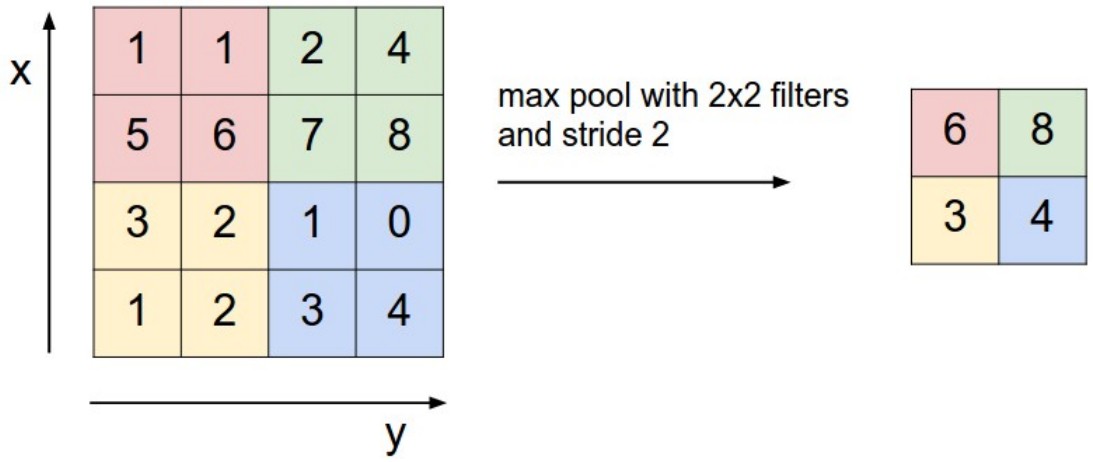
\includegraphics[scale=0.35]{./images/maxpool.png}
 \caption{\it Scheme of maxpool operations with a kernel of size $2 \times 2$ and stride $2$ over an image of size $4 \times 4$. Picture from CS231n}
 \label{fig:maxpool}
\end{figure}

The latter instead, returns the average value of the window and can be seen as a convolution where every weight in the kernel is $\frac{1}{k_x \cdot k_y}$.
The results expected from an Average pooling operations are shown in figure \ref{fig:avgpool:ex}:

\begin{figure}[h]
 \centering
 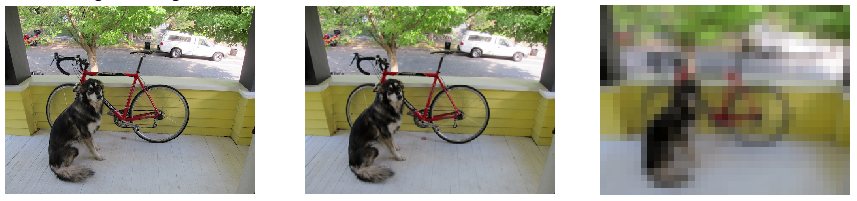
\includegraphics[scale=0.7]{./images/avgpool_layer.png}
 \caption{\it Average pooling applied to a test image: (left) the original image, (center) average pooling with a $3 \times 3$ kernel, (right) average pooling with a $30 \times 30$ kernel. The images have been obtained using NumPyNet}
 \label{fig:avgpool:ex}
\end{figure}

Other popular pooling functions include the $L^2$ norm of a rectangular neighborhood or a weighted average based on the distance from the central pixel.

A typical block of a convolutional network consists of three stages: In the first stage a CL performs several convolutions in parallel, in the second stage each convolution result is run through a non-linear activation function (sometimes called {\it detector}) and in the third stage a pooling function is used to further modify the output. 
The modification brought by pooling is helpful in different ways: first of all, it is a straightforward computational performance improvement, since less features also means less operations. 
Moreover, in all cases, pooling helps to make representation approximately invariant to small translation of the input and invariance to local translation can be a useful property if the objective is to decide wether a feature is present rather than where it is located \cite{Goodfellow-et-al-2016}.
The reductions of features can also prevent over-fitting problems during training, improving the general performances of the model. 

A pooling layer is defined by the same parameters as a CL, minus the number of filters:

\begin{itemize}
 \setlength\itemsep{-0.2em}
 \item [-] {\bf kernel size} : it is the size of the sliding filters. The depth of the filters is decided by the depth of the input images (which is the number of channels.). The remanining 2 dimensions (widht and height) can be indipendent from one another, but most implementations require square kernels.
 \item [-] {\bf strides} : defines the movement of the filters. With a low stride (e.g. unitary) the windows tends to overlap. With higher stride values we have less overlap (or none) and the dimension of the output decrease. Usually pooling operations have a stride of 2.
 \item [-] {\bf padding} : is the dimensions of an artificial enlargement of the input to allow the application of filters on borders. Usually, it can be interpreted as the number of rows/columns of pixel to add to the input, however some libraries (e.g Keras) consider it only as binary: in case is true, only the minimum number of rows/columns are appended to keep the same spatial dimension. Most often than not, no padding is applied during pooling operations.
\end{itemize}

The output dimensions for Pooling layers are the same as for CLs, however, since the operations does not change during the training phase, they have no weights.

Due to the similarities with the CL it is possible to implement a pooling layers through the im2col algorithm, as an example, the NumPyNet implementation shown in the snippet below make use of the function \texttt{asStride} to create a \texttt{view} of the input array: 

\lstset{style=snippet}
\begin{lstlisting}[language=Python, caption=NumPyNet version of AvgPool function, label=code:py_avgpool]
import numpy as np

class Avgpool_layer(object):

  def __init__(self, size=(3, 3), stride=(2, 2)):

    self.size = size
    self.stride = stride
    self.batch, self.w, self.h, self.c = (0, 0, 0, 0)
    self.output, self.delta = (None, None)

  def _asStride(self, input, size, stride):

    batch_stride, s0, s1 = input.strides[:3]
    batch,        w,  h  = input.shape[:3]
    kx, ky     = size
    st1, st2   = stride

    # Shape of the final view
    view_shape = (batch, 1 + (w - kx)//st1, 1 + (h - ky)//st2) + input.shape[3:] + (kx, ky)

    # strides of the final view
    strides = (batch_stride, st1 * s0, st2 * s1) + input.strides[3:] + (s0, s1)

    subs = np.lib.stride_tricks.as_strided(input, view_shape, strides=strides)
    # returns a view with shape = (batch, out_w, out_h, out_c, kx, ky)
    return subs

  def forward(self, input):

    self.batch, self.w, self.h, self.c = input.shape
    kx, ky = self.size
    sx, sy = self.stride

    input = input[:, : (self.w - kx) // sx*sx + kx, : (self.h - ky) // sy*sy + ky, ...]
    # 'view' is the strided input image, shape = (batch, out_w, out_h, out_c, kx, ky)
    view = self._asStride(input, self.size, self.stride)

    # Mean of every sub matrix, computed without considering the pad(np.nan)
    self.output = np.nanmean(view, axis=(4, 5))

\end{lstlisting}

A \texttt{view} is a special \texttt{numpy} object which retains the same information of the original array arranged in a different way, but without occupying more memory. In this case, the re-arrengement is very similar to an im2col, with the only differece that we are not bound to any number of dimensions. The resulting tensor has indeed 6 dimensions.
Since no copy is produces in this operation we can obtain a faster execution.

In pooling layer the backward function is similar to what we saw for convolutional layers, this time we don't have to compute the weights updates though, only the error to backprogate along the network.
For maxpool layers, only the maximum input pixel for every window is involved in the backward pass. Indeed, if we consider the simple case in which the forward function is : 

\begin{equation}
 m = max(a, b)
\end{equation}

and, as described in the dedicated chapter, we know that $\frac{\partial C}{\partial m}$ is the error passed back from the next layer: the objective is to compute $\frac{\partial C}{\partial a}$ and $\frac{\partial C}{\partial b}$. 
If $a > b$ we have : 

\begin{equation}
 m = a \quad \Rightarrow \quad \frac{\partial C}{\partial m} = \frac{\partial C}{\partial a}
\end{equation}
$m$ does not depends on $b$ so $\frac{\partial C}{\partial b} = 0$.

So the error is passed only to those pixel which value is maximum in the considered window, the other are zeros. 
In figure \ref{fig:maxpool:ex} an example of forward and backward pass for a maxpool kernel of size 30 and stride 20.

\begin{figure}[h]
 \centering
 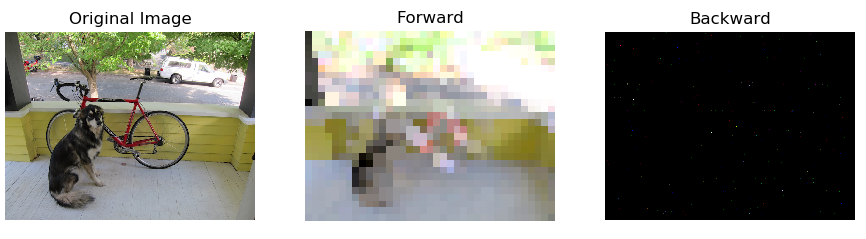
\includegraphics[scale=0.53]{./images/maxpool_30_20.png}
 \caption{\it Max pooling applied to a test image: (left) the original image, (center) max pooling with a $30 \times 3$0 kernel and stride $20$, (right) max pooling errors image. Only few of the pixels are responsible for the error backpropagation. 
 The images have been obtained using NumPyNet}
 \label{fig:maxpool:ex}
\end{figure}

The backward pass for the average pool layer is the same as for the CL, considering that in this case the "weights" are fixed.

% According to \cite{nopool}, it is possible to build models exclusively out of convolutional layers without the need for pooling and reach state-of-the art performances 

\subsection*{Shortcut Connections}

An important advancement in network architecture has been brought by the introduction of Shortcut (or Residual) Connections \cite{residual}. Famously, deep models suffer from {\it degradation problems} after reaching a maximum depth. Adding more layers, thus increasing the depth of the model, saturates the accuracy which eventually starts to rapidly decrease. 
The main cause of this dergradation is not overfitting, but numerical instability tied to gradient backpropagation: indeed, as the gradient is back-propagated through the network, repeated multiplications can make those gradients very small or, alternatevely, very big,
This problem is well known in Deep Learning and takes the name of {\it vanishing}/{\it exploding gradients} and it makes almost impossible to train very large models, since early layers may not learn anything even after hundreds of epochs.
A residual connection is a special shortcut which connects 2 different part of the network with a simple lnear combination.
Instead of learning a function $F(x)$ we try to learn $H(x) = F(x) + x$, as shown in figure \ref{fig:shortcut}:

\begin{figure}[h]
 \centering
 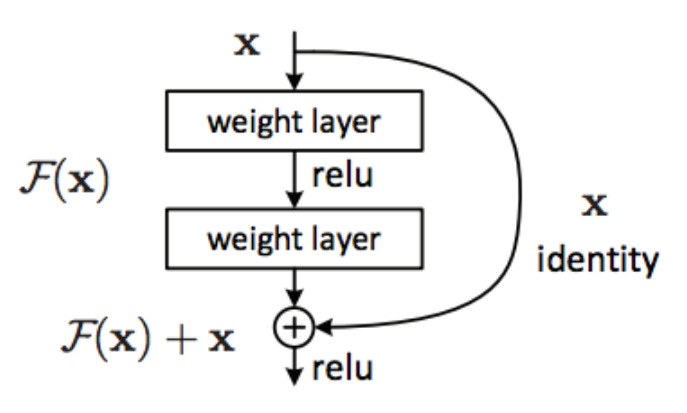
\includegraphics[scale=0.4]{./images/shortcut.png}
 \caption{\it Scheme of the shortcut layer as designed by the authors \cite{residual}. The output of the second layer become a linear combination of the input x and its own output.}
 \label{fig:shortcut}
\end{figure}
During the back propagation the gradient of higher layers can easily pass to the lower layers, without being mediated, which may cause vanishing or exploding gradient.
\\
Even the shortcut connection can be implemented as a stand-alone layer, defined by the following parameters:

\begin{itemize}
 \setlength\itemsep{-0.2em}
 \item {\bf index} is the index of the second input of this layer $x_2$ (the first one $x_1$ is the output of the previous layer).
 \item {\bf alpha} the first coefficient of the linear combination, multiplied by $x_1$.
 \item {\bf beta} the second coefficient of the linear combination, multiplied by $x_2$.
\end{itemize}
Both in NumPyNet and Byron, we chose to generalize the formula as: 

\begin{equation}
 H(x_1, x_2) = \alpha x_1 + \beta x_2
\end{equation}
Where $x_1$ is the output of the previous layer and $x_2$ is the output of the layer selected by \texttt{index}.
The backward function is simply :

\begin{equation}
 \frac{\partial C}{\partial x_1} = \frac{\partial C}{\partial H}\frac{\partial H}{\partial x_1} = \delta \cdot \alpha
\end{equation}
for the first layer and :

\begin{equation}
 \frac{\partial C}{\partial x_2} = \frac{\partial C}{\partial H}\frac{\partial H}{\partial x_2} = \delta \cdot \beta
\end{equation}
for the second layer. Again, $\delta$ is the error backpropagated from the next layer. 
Residuals connections were first introduced for image classification problems, but they rapidly become part of numerous models for every kind of application tied to Image Analysis.

\subsection*{Pixel Shuffle}

Using pooling and convolutional layers with non unitarian strides is a simple way to downsample the input dimension. 
For some applications though, we may be interested in upsampling the input, for example : 

\begin{itemize}
 \setlength\itemsep{-0.2em}
 \item in image to image processing (input and output are images of the same size) it is common to perform a compression to an internal encoding (e.g Deblurring, U-Net Segmentation). 
 \item project feature maps to a higher dimensional space, i.d. to obtain a image of higher resolution (e.g Super-Resolution)
\end{itemize}
for this purposes the {\it transposed convolution} (also called {\it deconvolution}) was introduced. 
The transposed convolution can be treated as a normal convolution with a sub-unitarian stride, by upsampling the input with empty rows and columns and then apply a single strided convolution, as shown in figure \ref{fig:deconv}:

\begin{figure}[h]
 \centering
 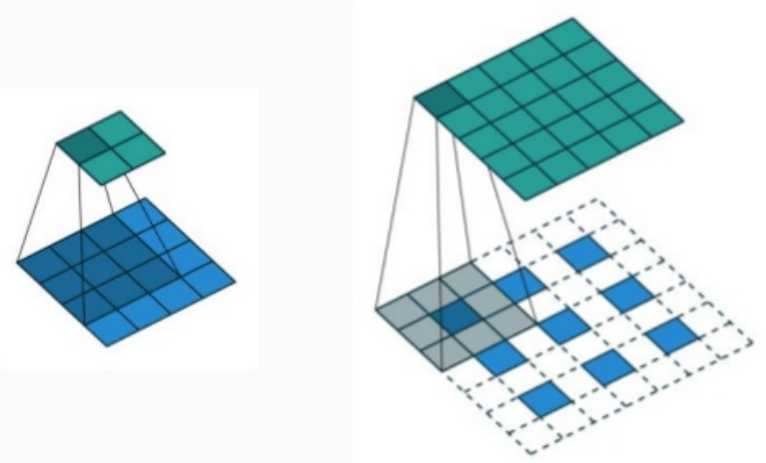
\includegraphics[scale=0.35]{./images/deconv.png}
 \caption{\it example of deconvolution: (left) a normal convolution with size 3 and stride 1, (right) after applying a "zeros upsampling" the convolution of size 3 and stride 1 become a deconvolution}
 \label{fig:deconv}
\end{figure}

Although working, the transposed convolution is not efficient in terms of computational and memory cost, therefore not suited for modern convolutional neural network. 
An alternative is the recently introduced {\it sub-pixel convolution} \cite{pixelshuffle} (also called Pixel Shuffle). The main advantages over the deconvolution operation is the absece of weights to train: indeed the operation perfermod by the Pixel Shuffle (PS) Layer is deterministic and it is very efficient if compared to the deconvolution, since it only performs a re-arrengement of the pixels. 

Given a scale factor $r$, the PS organizes an input $H \times W \times C \cdot r^2$ into an output tensor $r \cdot H \times r \cdot W \times C$, which generally is the dimension of the high resolution space. 
So, strictly speaking, the PS does not perform any upsample, since the number of pixels stays the same. 
In figure \ref{fig:pixelshuffle1} is shown an example with $C=1$:

\begin{figure}[h]
 \centering
 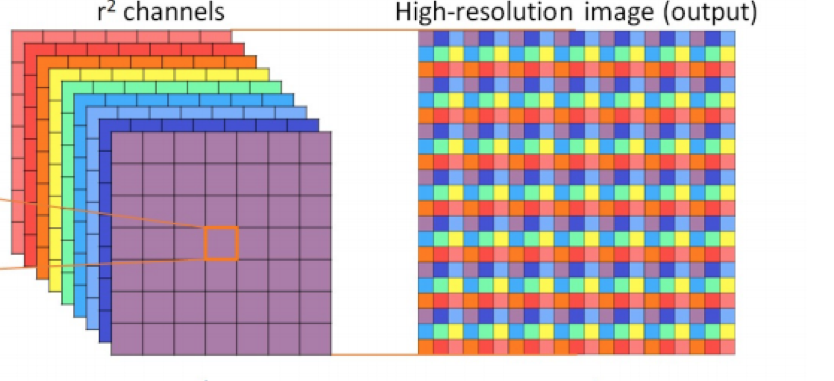
\includegraphics[scale=0.35]{./images/pixelshuffle.png}
 \caption{\it Example of pixel shuffling proposed by the authors \cite{pixelshuffle}. In this example, $r^2$ features maps are re-arranged into a single-channeled high resolution output.}
 \label{fig:pixelshuffle1}
\end{figure}

As suggested by the authors, the best practice to improve performances is to upscale from low resolution to High resolution only at the very end of the model. 
In this way the CL can efficienlty produce an high number of low resolution feature maps that the PS can organize into the final output. 

In both NumPyNet and Byron, the pixel shuffle layer is defined only by the \texttt{scale} parameter, which lead the entire transformation.
in the first case, it is possible to implement forward and backward using the functions \texttt{split}, \texttt{reshape}, \texttt{concatenate} and \texttt{transpose} of the \texttt{numpy} library \cite{Numpy}. 
This implementation has been tested against \texttt{tensorflow}'s \texttt{depth\_to\_space} and \texttt{space\_to\_depth}.
Despite beign available in most deep learning library, a low level  \texttt{C++} implementation for the PS algorithm is hard to find. 
In Byron we propose a dynamic algorithm able to work for both \texttt{channel last} and \texttt{channel first} input. 
The algorithm is essentially a re-indexing of the input array in six nested for-loops. The first soulution taken into account during the development was the contraction of the loops into a single one using divisions to obtain the correct indexes: however the amount of required divisions weights on the computational performances, given that divisions are the most expensive in terms of CPU clock-cycles. 

The backward function of this layer does not involve any gradient computation: instead, it is the inverse of the re-arrengement performed in the forward function.

\subsection*{Batch Normalization}

When training a neural network, the standard approach is to separate the dataset in groups, called {\it batches} or {\it mini-batches}. 
In this way the network can be trained with multiple input at a time and the updates for the weights are usually computed by averaging in the batch.
The number of examples in each batch is called \textit{batch size}: this can varies from 1 to the size of the dataset. 
Using batch sizes different from one is beneficial in several ways. 
First, the gradient of the loss over a mini-batch is a better estimate of the gradient over the train set, whose quality improves as the batch size increases, but using the entire train set can be very costly in terms of memory usage and often impossible to achieve.
Second, it can be much more efficient in modern architecture due to the  parallelism instead of performing M sequential computations for single examples. \cite{batchnorm}

Batch normalization is the operation that normalizes the features of the input along the batch axis, which allows to overcome a phenomenon in Deep Network training called {\it internal covariate shift}: whenever the parameters of the model change, the input distributions of every layer change accordingly.
This behaviour produces a slow down in the training convergence because each layer has to adapt itself to a new distribution of data for each epoch. Moreover, the parameters must be carefully initialized. 
By making the normalization a part of the model architecture, the layer acts also as a regularizer, which in turn allows better generalization perfomances.  

Let's $M$ be the number of examples in the group and $\epsilon$ a small variable added for numerical stability, the batch normalization function is defined as: 

\begin{align}
  &\mu = \frac{1}{M} \sum_{i=1}^{M} x_i \\
  &\sigma^2 = \frac{1}{M} \sum_{i=1}^{M} (x_i - \mu)^2 \\
  &\hat x_i = \frac{(x_i - \mu)^2}{\sqrt{\sigma^2 + \epsilon}} \\
  &y_i = \gamma \bar x_i + \beta
\end{align}

where $\gamma$ and $\beta$ are the trainable weights of this layer. In the case of a tensor of images of size $M \times H \times W \times C$ all the quantities are multidimensional tensor as well and all the operations are performed element-wise.

The backward function can be computed following the chain rule for derivatives. As usual, define $\delta^l = \frac{\partial C}{\partial y}$ as the error coming from the next layer, the goal is to compute the updates for $\gamma$ and $\beta$ and the error for the previous layer. 
The updates are straightforward: 

\begin{align}
 &\frac{\partial C}{\partial \gamma} = \frac{\partial C}{\partial y_i} \cdot \frac{\partial y_i}{\partial \gamma} = \sum_{i=1}^{M} \delta_i^l \cdot \hat x_i \\
 &\frac{\partial C}{\partial \beta} = \frac{\partial C}{\partial y_i} \cdot \frac{\partial y_i}{\partial \beta} = \sum_{i=1}^M \delta_i^l 
\end{align}

while the error requires more steps:

\begin{equation}
 \frac{\partial C}{\partial x} := \delta^{l-1} = \delta^l \cdot \frac{\partial y}{\partial  x}
\end{equation}

where : 

\begin{align}
 \frac{\partial y}{\partial x} = \frac{\partial y}{\partial \hat x} 
 (\frac{\partial \hat x}{\partial \mu}\frac{\partial \mu}{\partial x} + 
  \frac{\partial \hat x}{\partial \sigma^2}\frac{\partial \sigma^2}{\partial x} +
\frac{\partial \hat x}{\partial \sigma^2}\frac{\partial \sigma^2}{\partial \mu}\frac{\partial \mu}{\partial x})
\end{align}

By considering all the derivatives, we find :

\begin{equation}
 \frac{\partial C}{\partial x_i} := \delta^{l-1}_i = 
 \frac{M\delta^l_i \cdot \gamma_i - \sum_{j=1}^{M} \delta^l_j \cdot \gamma_i - \hat x_i \cdot \sum_{j=1}^{M} \delta^l_j \cdot \hat x_j}
 {M\sqrt{\sigma^2 + \epsilon}}
\end{equation}

Knowing the correct operations, an example of implementation is shown in the snippet \ref{code:py_batchnorm}: 

\lstset{style=snippet}
\begin{lstlisting}[language=Python, caption=NumPyNet version of batchnorm function, label=code:py_batchnorm]

def forward(self, inpt):
  '''
  Forward function of the BatchNormalization layer. It computes the output of
  the layer, the formula is :
                  output = scale * input_norm + bias
  Where input_norm is:
                  input_norm = (input - mean) / sqrt(var + epsil)
  where mean and var are the mean and the variance of the input batch of
  images computed over the first axis (batch)
  Parameters:
    inpt  : numpy array, batch of input images in the format (batch, w, h, c)
  '''

  self._check_dims(shape=self.input_shape, arr=inpt, func='Forward')

  # Copy input, compute mean and inverse variance with respect the batch axis
  self.x    = inpt.copy()
  self.mean = self.x.mean(axis=0)                             # shape = (w, h, c)
  self.var  = 1. / np.sqrt((self.x.var(axis=0)) + self.epsil) # shape = (w, h, c)
  # epsil is used to avoid divisions by zero

  # Compute the normalized input
  self.x_norm = (self.x - self.mean) * self.var # shape (batch, w, h, c)
  self.output = self.x_norm.copy() # made a copy to store x_norm, used in Backward

  # Init scales and bias if they are not initialized (ones and zeros)
  if self.scales is None:
    self.scales = np.ones(shape=self.out_shape[1:])

  if self.bias is None:
    self.bias = np.zeros(shape=self.out_shape[1:])

  # Output = scale * x_norm + bias
  self.output = self.output * self.scales + self.bias

  # output_shape = (batch, w, h, c)
  self.delta = np.zeros(shape=self.out_shape, dtype=float)

  return self

def backward(self, delta=None):
  '''
  BackPropagation function of the BatchNormalization layer. Every formula is a derivative
  computed by chain rules: dbeta = derivative of output w.r.t. bias, dgamma = derivative of
  output w.r.t. scales etc...
  Parameters:
    delta : the global error to be backpropagated, its shape should be the same
      as the input of the forward function (batch, w, h ,c)
  '''

  check_is_fitted(self, 'delta')
  self._check_dims(shape=self.input_shape, arr=delta, func='Forward')

  invN = 1. / np.prod(self.mean.shape)

  # Those are the explicit computation of every derivative involved in BackPropagation
  # of the batchNorm layer, where dbeta = dout / dbeta, dgamma = dout / dgamma etc...

  self.bias_update = self.delta.sum(axis=0)                   # dbeta
  self.scales_update = (self.delta * self.x_norm).sum(axis=0) # dgamma

  self.delta *= self.scales                                    # self.delta = dx_norm from now on

  self.mean_delta = (self.delta * (-self.var)).mean(axis=0)    # dmu

  self.var_delta = ((self.delta * (self.x - self.mean)).sum(axis=0) *
                    (-.5 * self.var * self.var * self.var))     # dvar

  # Here, delta is the derivative of the output w.r.t. input
  self.delta = (self.delta * self.var +
                self.var_delta * 2 * (self.x - self.mean) * invN +
                self.mean_delta * invN)

  if delta is not None:
    delta[:] += self.delta

  return self
  
\end{lstlisting}

As we can see, in \texttt{numpy} it's possible to easily implement all element-wise operations with standard algebra.

In \texttt{Byron} we decided to implement this operation both as a standalone function and merged into convolutional and fully connected layers, with the latter being the most used in modern models since it achieves the best computational performances.

\subsection*{Activations}

An important role in neural network is played by the choice of activation function.

\begin{itemize}
 \item table
 \item example images
 \item forward backward
\end{itemize}

\begin{table*}[h]
\centering
\begin{adjustbox}{max width=\textwidth}
\begin{tabular}{lcc}
\hline \rowcolor{darkgrayrow}
\textbf{Name} & \textbf{Equation} & \textbf{Derivative} \\
\hline

Linear   &  $f(x) = x$                              &  $f'(x) = 1$ \\

Logistic &  $f(x) = \frac{1}{1 + \exp(-x)}$         &  $f'(x) = (1 - f(x)) * f(x)$ \\

Loggy    &  $f(x) = \frac{2}{1 + \exp(-x)} - 1$     &  $f'(x) = 2 * (1 - \frac{f(x) + 1}{2}) * \frac{f(x) + 1}{2} $ \\

Relu     &  $f(x) = \max(0, x)$                     &  $f'(x) = \left\{\begin{array}{rlr}
                                                                       1   & \mbox{if} & f(x) > 0    \\
                                                                       0   & \mbox{if} & f(x) \leq 0
                                                                       \end{array}\right.$           \\

Elu      &  $f(x) = \max(\exp(x) - 1, x)$           &  $f'(x) = \left\{\begin{array}{rlr}
                                                                       1        & \mbox{if} & f(x) \geq 0 \\
                                                                       f(x) + 1 & \mbox{if} & f(x) < 0
                                                                       \end{array}\right.$                \\

Relie    &  $f(x) = \max(x * 1e-2, x) $             &  $f'(x) = \left\{\begin{array}{rlr}
                                                                       1    & \mbox{if} & f(x) > 0    \\
                                                                       1e-2 & \mbox{if} & f(x) \leq 0
                                                                       \end{array}\right.$            \\

Ramp     &  $f(x) = \left\{\begin{array}{rlr}
                            x^2 + 0.1 * x^2 &  \mbox{if} & x > 0    \\
                            0               &  \mbox{if} & x \leq 0
                           \end{array}\right.$
                                                    &  $f'(x) = \left\{\begin{array}{rlr}
                                                                       f(x) + 1 & \mbox{if} & f(x) > 0   \\
                                                                       f(x)     & \mbox{if} & f(x) \leq 0
                                                                       \end{array}\right.$               \\

Tanh     &  $f(x) = \tanh(x)$                       &  $f'(x) = 1 - f(x)^2$  \\

Plse     &  $f(x) = \left\{\begin{array}{rlr}
                            (x + 4) * 1e-2     & \mbox{if} & x < -4           \\
                            (x - 4) * 1e-2 + 1 & \mbox{if} & x > 4            \\
                            x * 0.125 + 5      & \mbox{if} & -4 \leq x \leq 4
                           \end{array}\right.$
                                                    &  $f'(x) = \left\{\begin{array}{rlr}
                                                                       1e-2  & \mbox{if } & f(x) < 0 \mbox{ or } f(x) > 1 \\
                                                                       0.125 & \mbox{if } & 0 \leq f(x) \leq 1
                                                                       \end{array}\right.$                                \\

Leaky    &  $f(x) = \left\{\begin{array}{rlr}
                            x * C &  \mbox{if} & x \leq 0 \\
                            x     &  \mbox{if} & x > 0
                           \end{array}\right.$
                                                    &  $f'(x) = \left\{\begin{array}{rlr}
                                                                       1   & \mbox{if} & f(x) > 0    \\
                                                                       C   & \mbox{if} & f(x) \leq 0
                                                                       \end{array}\right.$           \\

HardTan  &  $f(x) = \left\{\begin{array}{rlr}
                            -1 & \mbox{if} &     x < -1 \\
                            +1 & \mbox{if} &     x > 1  \\
                             x & \mbox{if} & -1 \leq x \leq 1
                           \end{array}\right.$
                                                    &  $f'(x) = \left\{\begin{array}{rlr}
                                                                        0 & \mbox{if} & f(x) < -1 \mbox{ or } f(x) > 1 \\
                                                                        1 & \mbox{if} & -1 \leq f(x) \leq 1
                                                                       \end{array}\right.$                            \\

LhTan    &  $f(x) = \left\{\begin{array}{rlr}
                            x * 1e-3           & \mbox{if} &     x < 0  \\
                            (x - 1) * 1e-3 + 1 & \mbox{if} &     x > 1  \\
                             x                 & \mbox{if} & 0 \leq x \leq 1
                           \end{array}\right.$
                                                    &  $f'(x) = \left\{\begin{array}{rlr}
                                                                        1e-3           & \mbox{if} & f(x) < 0 \mbox{ or } f(x) > 1 \\
                                                                        1              & \mbox{if} & 0 \leq f(x) \leq 1
                                                                       \end{array}\right.$                                  \\

Selu     &  $f(x) =\left\{\begin{array}{rlr}
                            1.0507 * 1.6732 * (e^x - 1) & \mbox{if} &    x < 0  \\
                            x * 1.0507                  & \mbox{if} &    x \geq 0
                           \end{array}\right.$

                                                    &  $f'(x) = \left\{\begin{array}{rlr}
                                                                        f(x) * 1e-3           & \mbox{if} & f(x) 0    \\
                                                                        (f(x) - 1) * 1e-3 + 1 & \mbox{if} & f(x) > 1  \\
                                                                        \end{array}\right.$                           \\

SoftPlus &  $f(x) = log(1 + e^{x})$                 &  $f'(x) = \frac{\exp(f(x)}){1 + e^{f(x)}}$ \\

SoftSign &  $f(x) = \frac{x}{|x| + 1}$              &  $f'(x) = \frac{1}{(|f(x)| + 1)^{2}}$ \\

Elliot   &  $f(x) = \frac{\frac{1}{2} * S * x}{1 + |x + S|} + \frac{1}{2}$

                                                    &  $f'(x) = \frac{\frac{1}{2} * S}{(1 + |f(x) + S|)^{2}} $ \\

SymmElliot &  $f(x) = \frac{S * x}{1 + |x * S|}$    &  $f'(x) = \frac{S}{(1 + |f(x) * S|)^{2}}$ \\


%Swish    &  $f(x) = $                               &  $f'(x) = $                                                                                            %\\

%SoftMax  &  $f(x) =\frac{\exp(x)}{\sum_{i=1}^{N}x}$ &  $f'(x) = $


\hline\\
\end{tabular}
\end{adjustbox}
\caption{\it List of common activation functions with their corresponding mathematical equation and derivative.
The derivative is expressed as function of $f(x)$ to optimize their numerical evaluation.
}
\label{tab:activations}
\end{table*}

\subsection*{Loss Function}
\section{Timing}

\chapter{Datasets and Methodology}

\section{Models}

As already described in previous chapters, the high level of modularity provided by \texttt{Byron} and \texttt{NumPyNet} allows to use different kind of models for many different purposes. \\


\href{https://github.com/thstkdgus35/EDSR-PyTorch}{EDSR} \\
\href{https://github.com/JiahuiYu/wdsr_ntire2018}{WDSR}

\subsection*{EDSR}

\subsection*{WDSR}

\section{Train Dataset : DIV2K}

The training set is a general purpose dataset called DIV2K \cite{DIV2K} and it has been employed to train and validate {\tt EDSR} and {\tt WDSR} for the {\it NTIRE} competition (New Trends in Image Restoration and Enhancement).

The dataset is composed by 1000 2K RGB images with a large diversity of contents, divided into:

\begin{itemize}
 \setlength\itemsep{-0.2em}
 \item {\bf Training set} : 800 HR images and 800 LR images obtained from the HR ones using different downscaling factor (2x, 3x, 4x) and different degrading factor.
 \item {\bf Validation set} : 100 HR images and 100 LR images used as a test set to evaluate the models by the competitors.
 \item {\bf Test set} : 100 LR images for which an HR version is made available only at the end of the competition. This is used by the competitors to test the models and for their final evaluation.
\end{itemize}

A qualitative proof of the results obtainable from the two models are shown in pictures \ref{fig:sky}, \ref{fig:city} and \ref{fig:windows}.

\begin{figure}[h!]
  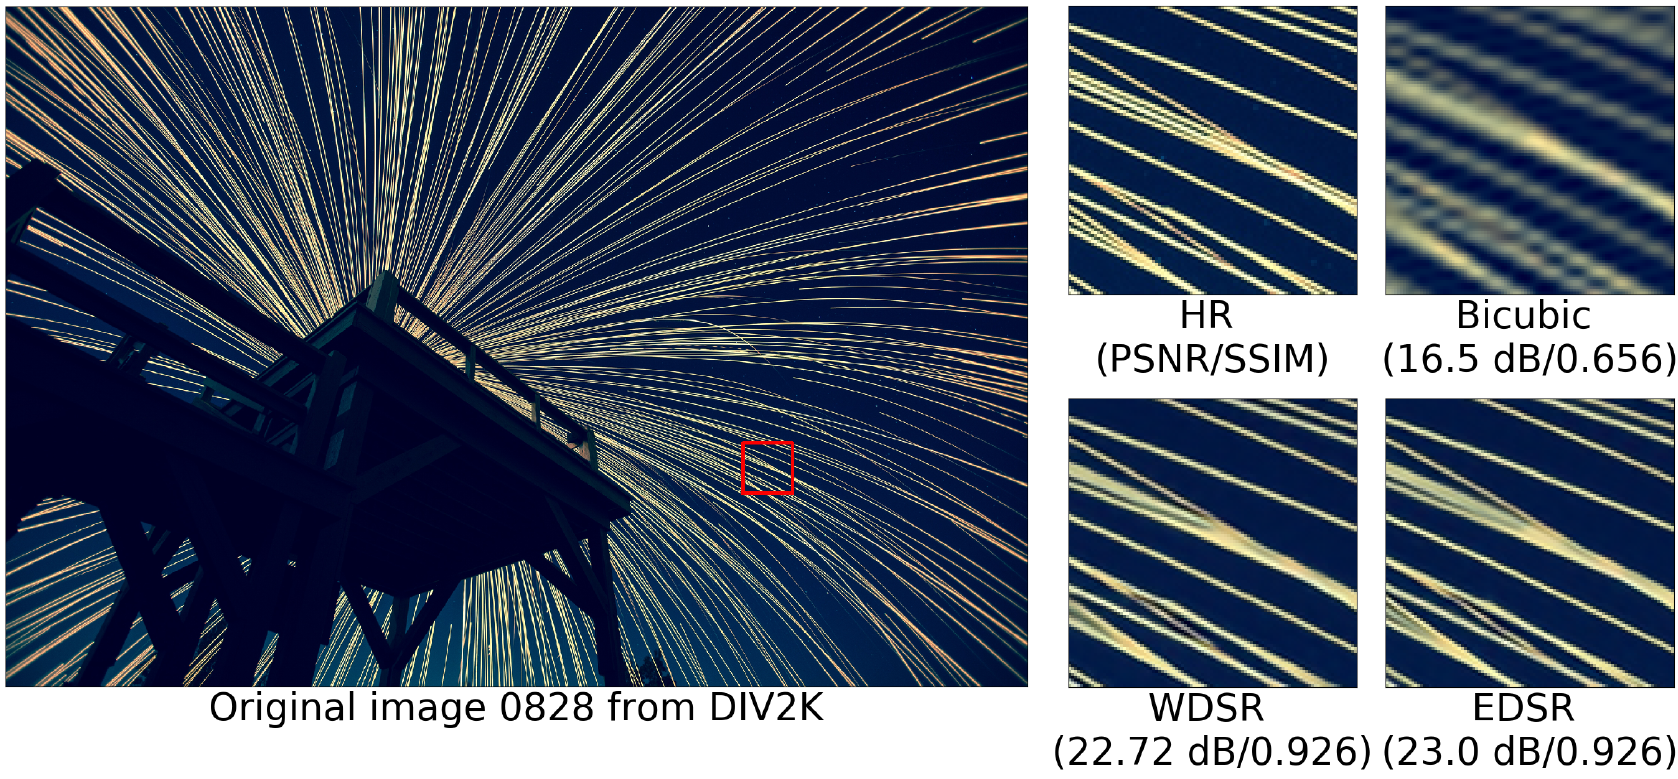
\includegraphics[scale=0.5]{images/sr_res1.png}
    \caption{\it Super Resolution visual example extracted from the DIV2K validation set. The quality score in terms of PSNR and SSIM are compared between a standard bi-cubic up-sampling and the EDSR and WDSR models.}
  \label{fig:sky}
\end{figure}

\begin{figure}[h!]
  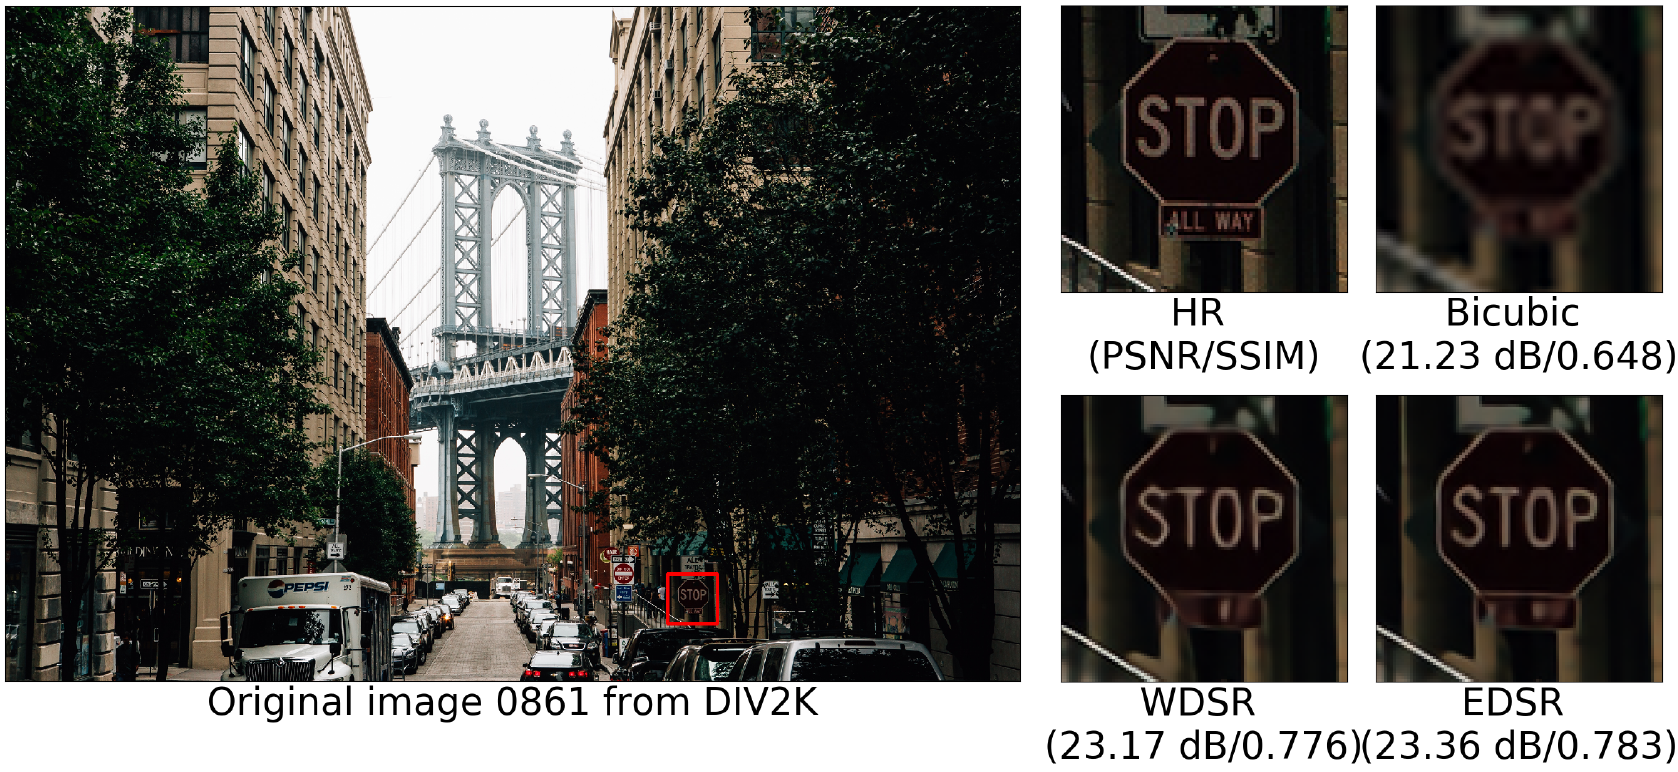
\includegraphics[scale=0.5]{images/sr_res2.png}
    \caption{\it Super Resolution visual example extracted from the DIV2K validation set. The quality score in terms of PSNR and SSIM are compared between a standard bi-cubic up-sampling and the EDSR and WDSR models.}
  \label{fig:city}
\end{figure}

\begin{figure}[h]
  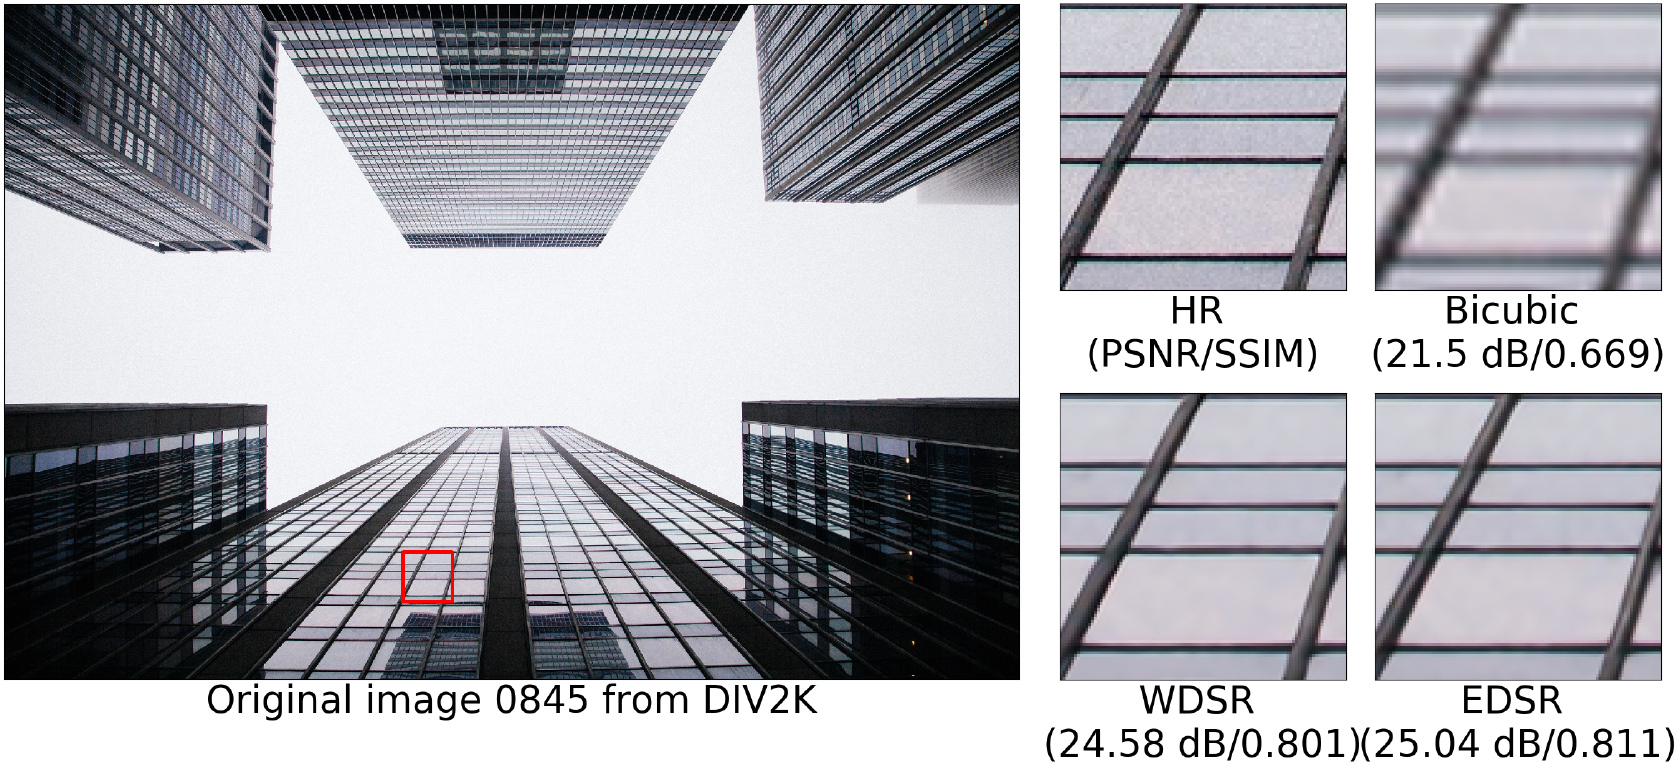
\includegraphics[scale=0.5]{images/sr_res3.png}
  \caption{\it Super Resolution visual example extracted from the DIV2K validation set. The quality score in terms of PSNR and SSIM are compared between a standard bi-cubic up-sampling and the EDSR and WDSR models.}
  \label{fig:windows}
\end{figure}

As can be seen in those pictures, the models have learned how to interpolate the complex line shapes and different kind of textures better that the bicubic algorithm.
Given the great heterogeneity of contents inside the dataset, after the training phase the models are able to reconstruct a huge amount of distict shapes and textures. For this reasons we decided to test the performances of {\tt WDSR} and {\tt EDSR} on a set of NMR data. 

\section{NMR Dataset}

To test the model on NMR images, we used a series of 5 patients weighted $T_1$ and $T_2$ sampled with a spatial frequency of $1mm \times 1mm \times 1mm$ for each direction ($x, y, z$), with a resolution of $256 \times 256$ for a total of 176 slices. For reference, in figure \ref{fig:orig_ref} are shown three different slices for the same patient at HR:

\begin{figure}[H]
 \centering
 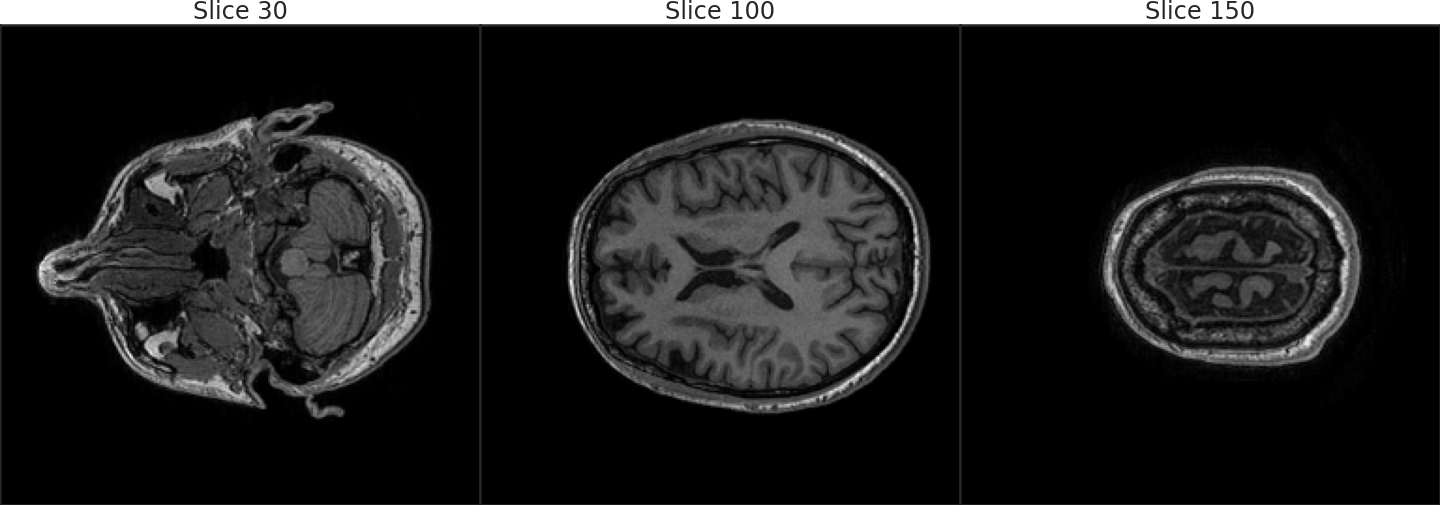
\includegraphics[scale=0.31]{./images/orig_slice_comp.png}
 \caption{\it HR $256 \times 256$ original image at three different stages of depth: (left) slice 30 where still a lot of information about the brain is hidden, (center) slice 100 which is a central slice where most of the information is stored, (right) slice 150 which starts the less informative area of the brain.}
 \label{fig:orig_ref}
\end{figure}

Then, the HR images (which will also be called {\it originals}) have been  downsampled with the bicubic algorithm by two different scale factors, namely 2x and 4x, obtaining two distinct sets of LR images for every subject and for every weight, respectively of sizes $128 \times 128 \times 176$ and $64 \times 64 \times 176$.

After all that, the LR images are convoluted with a gaussian kernel of size 3, stride 1 and standard deviation 1 with the function \texttt{cv2.GaussianBlur} of the library OpenCV. 
This has been done to better resemble a LR data-acquisition, as if the images were obtained at low resolution directly and not coming from a downsampling.
In figure \ref{fig:inp2} is shown an example of the images obtained by this procedure for a downscale factor of 2:

\begin{figure}[H]
 \centering
 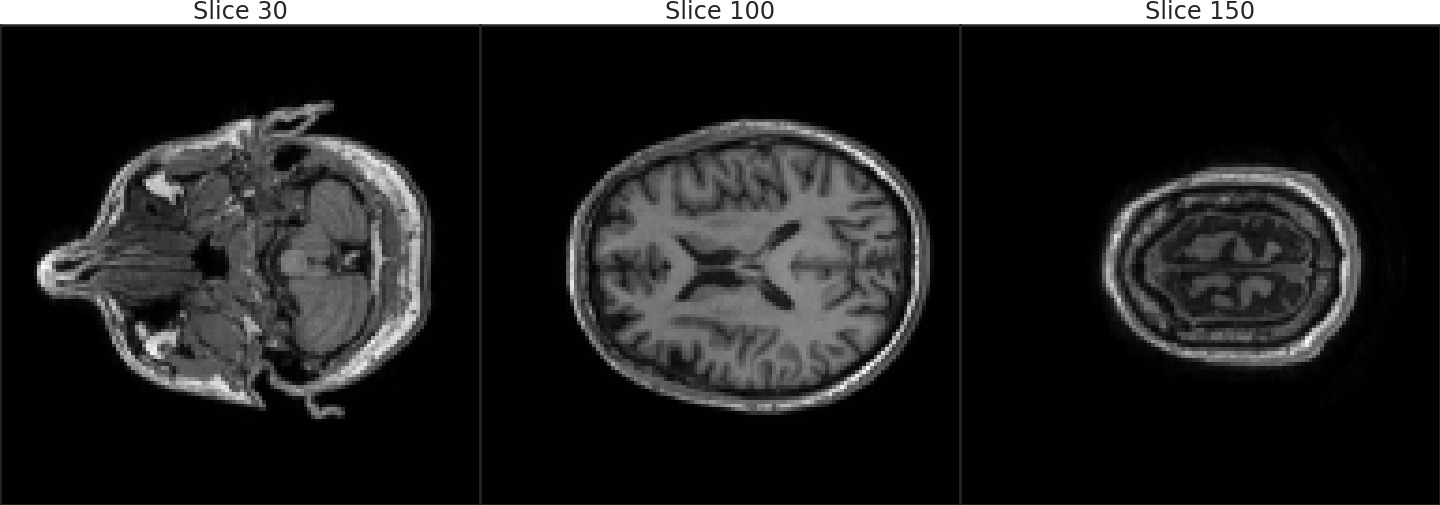
\includegraphics[scale=0.3]{images/inp2_slice_comp.png}
 \caption{\it $128 \times 128$ LR version of the same slices shown for the HR case.}
 \label{fig:inp2}
\end{figure}

In figure \ref{fig:inp4} is shown an example of the images obtained by this procedure for a downscale factor of 4:

\begin{figure}[H]
 \centering
 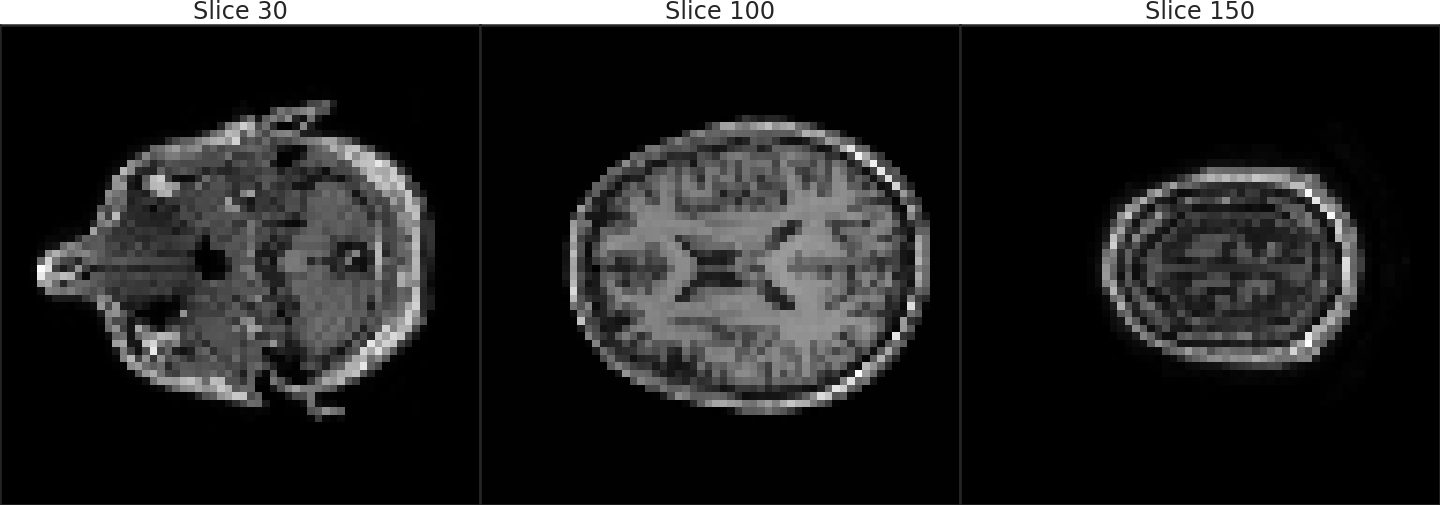
\includegraphics[scale=0.3]{images/inp4_slice_comp.png}
 \caption{\it $64 \times 64$ LR version of the same slices shown for the HR case.}
 \label{fig:inp4}
\end{figure}

The LR images are used as input for {\tt EDSR}, {\tt WDSR} and the bicubic algorithm which re-upsample them respectively by factors 2x, 4x and both, trying to recostruct an image as close as possible to the original one.
As further analysis we decided to investigate how different input conditions influence the results for the three methods. 
In particular how an angle of rotation for the input images can impact the final re-upsample: indeed this changes the orientation of lines, shapes and textures in the images and can change the reconstruction. 
Nonetheless it can give an important insight on the level of invariance of the two models and on the {\it explainability} of the results. 

I divided the full angle into 20 sections, separated by a step of $18$°. In figure \ref{fig:rotations} is shown an example of the kind of inputs fed to the models:

\begin{figure}[H]
 \centering
 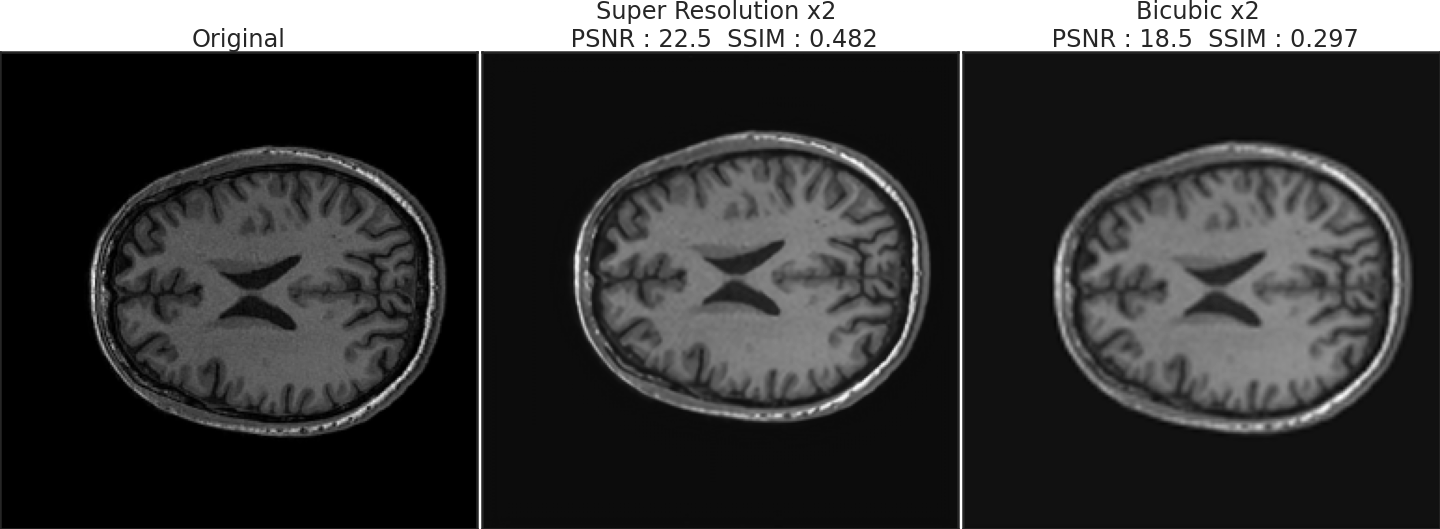
\includegraphics[scale=0.3]{images/rotations.png}
 \caption{\it Three of the 20 rotation angles used as input for Super Resolution models and Bicubic. (left) reference angle of 0 degree, (centre) angle step of 18 degree, (right) large rotation of 108° respect to the reference. }
 \label{fig:rotations}
\end{figure}

The recostruction are compared with the original images using PSNR and SSIM values for every patient, weight, channel, scale factor and angle of rotation. 
As stated before, the NMR slices are 1-channeled gray-scale image while the SR models work on RGB image: this is solved by adding an artificial depth concatenating the same slice 3 times. 
The dataset of original HR images is publicly available from \href{http://insight-journal.org/midas/collection/view/190}{MIDAS} \cite{dataset}. 

\chapter{Results}

In the following chapter I'm going to report quantitative and qualitative results for the different analysis carried out during the work.
I describe the quantitative results obtained by the different methods evaluated by means of PSNR, SSIM score and by a qualitative visual analisys.
At the end of the chapter I will summarize the results and provides possible continuations for future analysis.  

\section{Upsample Comparisons}

The {\tt EDSR} model is used to upsample the images by a x2 factor so that the single slice is Super Resolved from a $128 \times 128$ to a $256 \times 256$ spatial resolution. 
The {\tt WDSR} model instead, is used to upsample the images by a x4 factor so that the single slice is Super Resolved from a $64 \times 64$ to a $256 \times 256$ spatial resolution. 

I decided to separate the analysis for the three output channel of the super-resolution since it can highlight particular behaviours. 
In figure \ref{fig:edsr-score-slide} are shown the average trends for PSNR and SSIM score for the three channels (Red, Green, Blue lines) and for the bicubic algorithm (Yellow lines). 
It is clear that there is a difference between the three output for the super resolution: namely there is a vertical shift in the trends passing from Red to Blue and from Blue to Green, the latter being the best performer.
Moreover, the "best" channel for {\tt EDSR} outperforms consinstently the bicubic algorithm in the most informative section of the subjects.

\begin{figure}[H]
  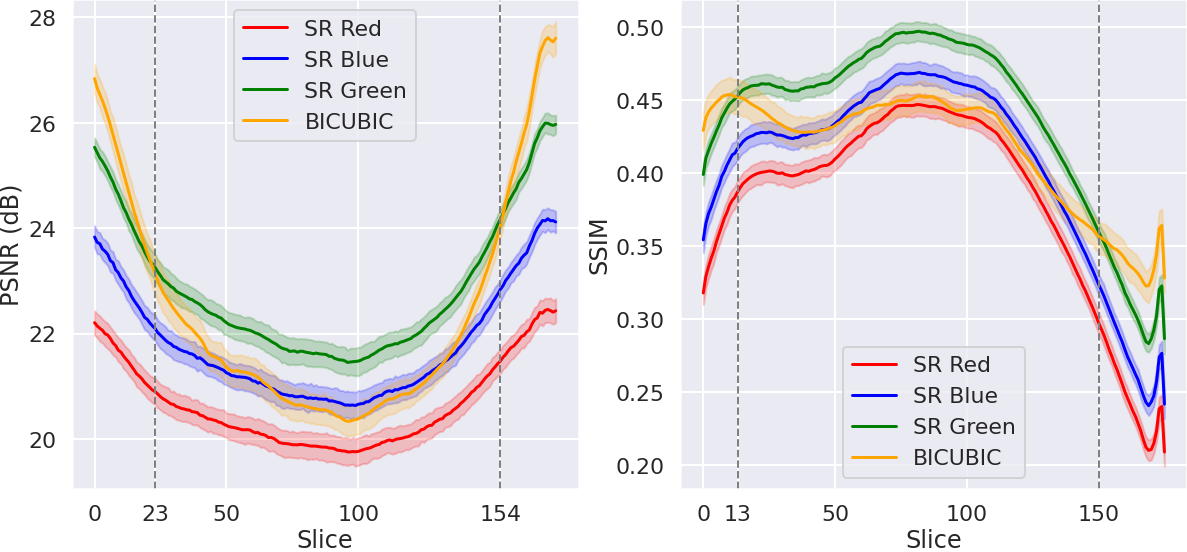
\includegraphics[scale=0.37]{./images/edsr_score_slide.png}
  \caption{\it Average trends of PSNR (left) and SSIM (right) for the three channels (Red, Blue, Green lines) of the Super Resolution EDSR model compared with the bicubic algorithm scores (Yellow) as functions of the slices. The average is performed for every patients and for every rotation. The dotted lines highlights the slices where the bicubic and Super Resolution performances intersect. The bicubic seems to perform better that SR only on the less informative section of the subjects.}
  \label{fig:edsr-score-slide}
\end{figure}

In figure \ref{fig:edsr-upscale} is shown an example on the kind of reconstruction the two methods are able to achieve on a significant slice : 

\begin{figure}[H]
 \centering
 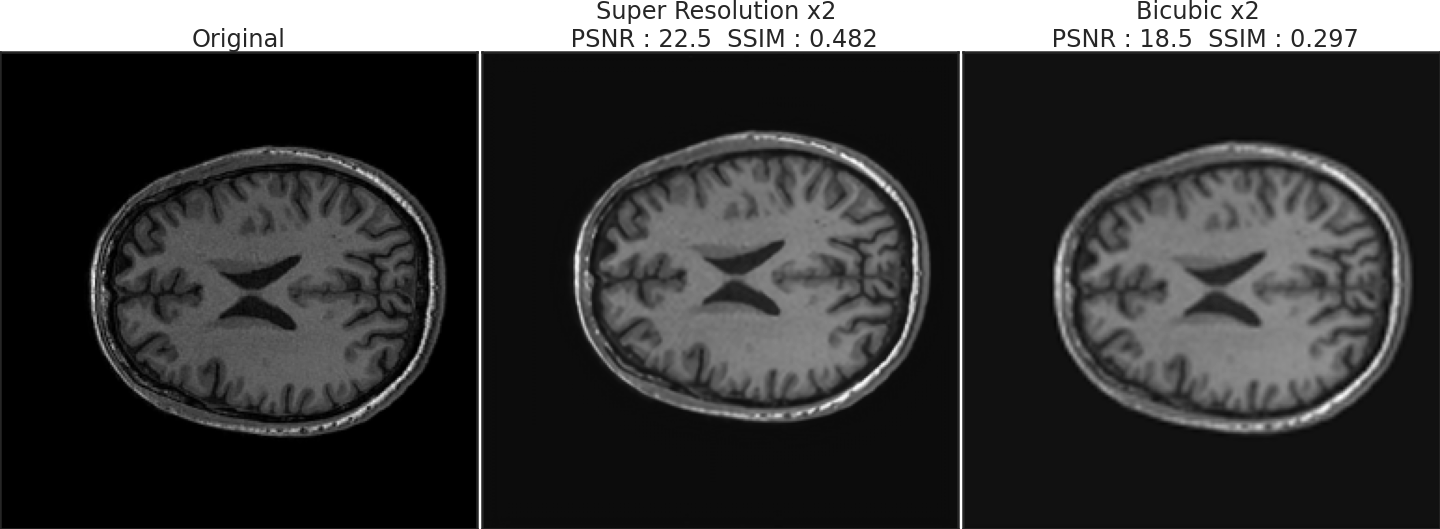
\includegraphics[scale=0.3]{./images/edsr-comp-images.png}
 \caption{\it (left) original image, (center) reconstruction performed with {\tt EDSR}, (right) reconstruction using the bicubic method. The input in this case is not rotated.}
 \label{fig:edsr-upscale}
\end{figure}

On the other hand, the three outputs of the {\tt WDSR} are more consistents between each others and through the subjects they performs, on average, steadily better than the bicubic algorithm. As shown in figure \ref{wdsr-score-slide}    

\begin{figure}[H]
  \centering
 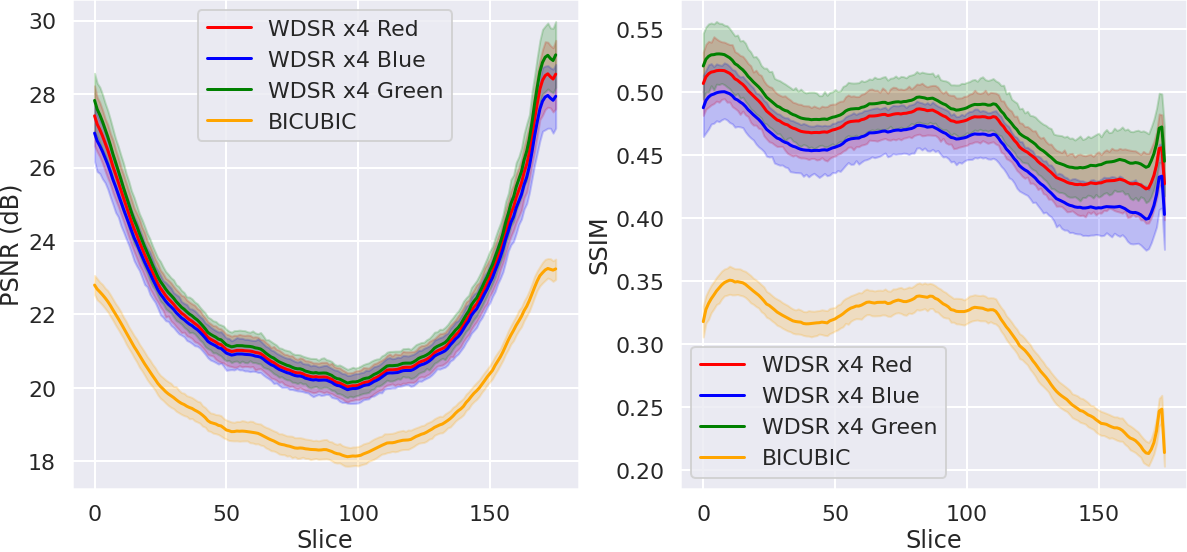
\includegraphics[scale=0.37]{./images/wdsr_score_slide.png}
  \caption{\it Average trends of PSNR (left) and SSIM (right) for the three channels (Red, Blue, Green lines) of the Super Resolution WDSR model compared with the bicubic algorithm scores (Yellow) as functions of the slices. The average is performed for every patients and for every rotation.}
 \label{fig:wdsr-score-slide}
\end{figure}

A recostruction performed starting from a donwscaled input $64 \times 64$ is shown in figure \ref{wdsr-upscale} for the two methods:

\begin{figure}[H]
 \centering
  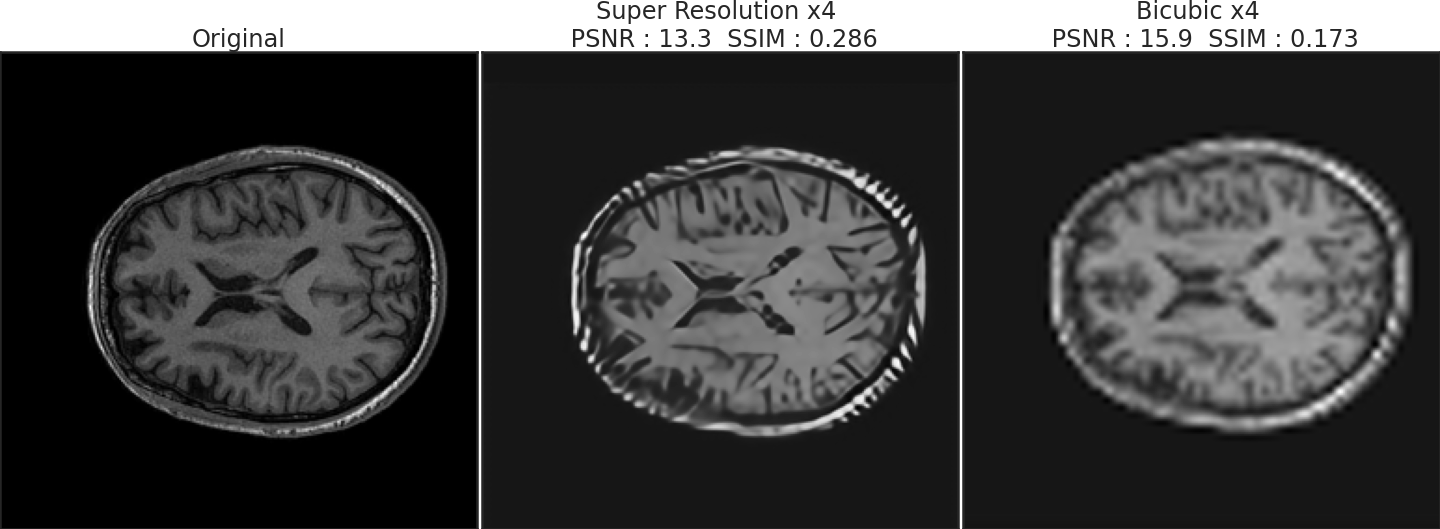
\includegraphics[scale=0.3]{images/wdsr-comp-images.png}
  \caption{\it (left) original image, (center) reconstruction performed with {\tt WDSR}, (right) reconstruction using the bicubic method. The input in this case is not rotated.}
 \label{wdsr-upscale}
\end{figure}

The result is clearly worst than the previous case since the x4 down-scaling is quite heavy.
In both cases the upsampling methods introduce a bias on the background of the image which can spoil the quantitative result.

\section{Scores By Angle}

The next analysis focused on how 

\begin{figure}[H]
 \centering
 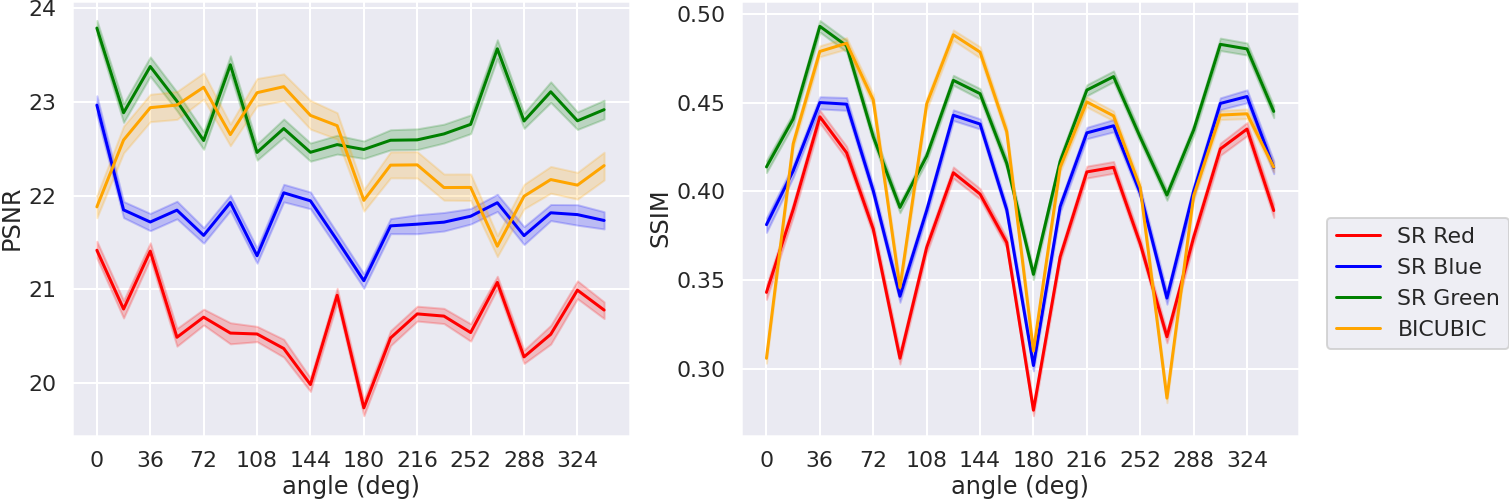
\includegraphics[scale=0.3]{./images/edsr-angles.png}
 \caption{\it edsr}
 \label{fig:edsr-angles}
\end{figure}


\begin{figure}[H]
 \centering
 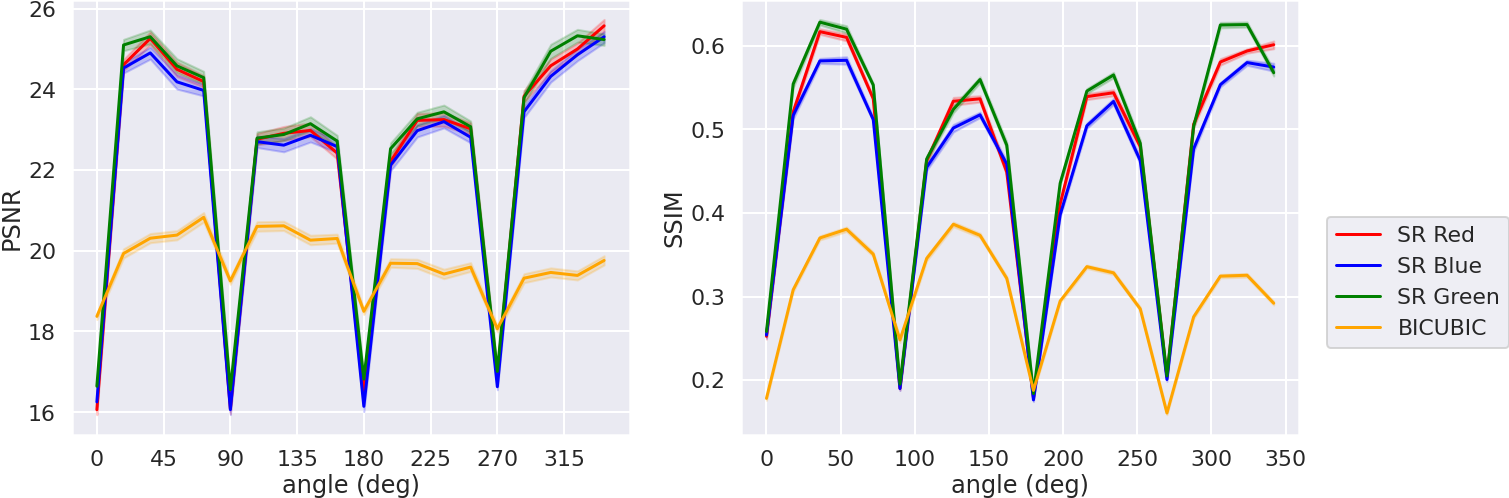
\includegraphics[scale=0.3]{./images/wdsr-angles.png}
 \caption{\it wdsr}
 \label{fig:edsr-angles}
\end{figure}

\begin{itemize}
 \setlength\itemsep{-0.2em}
 \item how the performances varies with angle
 \item comparisons of rotated angle reconstruction.
 \item where are located the differences 
 \item how is the difference distributed (histograms)
 \item difference between t1 and t2
 \item download some T2 case01015 images 
 \item Results without scalp
\end{itemize}


\section{}

\section{Conclusions}


\newpage
\thispagestyle{empty}
\listoffigures

\newpage
\nocite{*}
\bibliographystyle{abbrv}
\bibliography{biblio}

\end{document}
